% This is supposed to be the submitted version.
%   Remove reference to p-curve 2.1 being demonstrably more accurate than 6.04 -- for the present.
%   

%% -----------------------------------------------------------------------------
%% Uses bibtex file power6.bib
%% Run LaTeX, then BibTeX, then LaTeX again. Need to run BibTeX every time 
%% the references are modified. In TeXShop preferences under Engine, the BibTeX Engine 
%% should be biber. Re-set after installing a new version of LaTeX.
%% ----------------------------------------------------------------------

\documentclass[jou]{apa6} % Other options are man (for manuscript) and doc for a more normal LTeX document.

\usepackage[american]{babel}

\usepackage{csquotes}
\usepackage[style=apa,sortcites=true,sorting=nyt,backend=biber]{biblatex}
\DeclareLanguageMapping{american}{american-apa}
\addbibresource{zcurve6.bib}


%%%%%%%%%%%%%%%%%%%%%%%%%%%%%% Jerry's preamble additions %%%%%%%%%%%%%%%%%%%%%%%%%%%%%%

\newtheorem{princ}{Principle}           
\usepackage{amsbsy} % for \boldsymbol and \pmb 
\usepackage{amsmath}       
\usepackage{graphicx} % For example, 
\includegraphics[width=3in]{density1}
\usepackage{graphpap}
\usepackage{float} % For unconditional H placement of figures and tables
\usepackage{amssymb} % for \blacksquare
\usepackage{euscript} % for \EuScript
%\usepackage[colorlinks=true, pdfstartview=FitV, linkcolor=blue, citecolor=blue, urlcolor=blue]{hyperref} % For links
\usepackage[colorlinks=true, pdfstartview=FitV, linkcolor=blue, citecolor=black, urlcolor=blue]{hyperref} % For links
\usepackage{setspace}
% \doublespacing % For manuscript mode

\newcommand{\R}[1]{\mbox{\texttt{#1}}} % To typeset R-like syntax in math mode.
% \numberwithin{equation}{section}

% Lovely examples of bibtex, apa6
%                       CODE                                          OUTPUT
% \parencite{Bunge1998, Popper1959}                     (Bunge, 1998; Popper, 1959)
% \textcite{Cohen1962}                                  Cohen (1962)                    
% \parencite[for example,][p. 24]{Cohen1988}            (for example, Cohen, 1988, p. 24)
% \parencite[][Ch.~6]{LehmanCasella1998}                (Lehman & Casella, 1998, Ch. 6)
% \citeauthor{Cohen1962}'s (\citeyear{Cohen1962}) classic       Cohen’s (1962) classic

%%%%%%%%%%%%%%%%%%%%%%%%%%%%%%%%%%%%%%%%%%%%%%%%%%%%%%%%%%%%%%%%%%%%%%%%%%%%%%


\title{Estimating Population Mean Power Under Conditions of Heterogeneity and Selection for Significance}
\shorttitle{Estimating Mean Power}

\author{Jerry Brunner and Ulrich Schimmack}
\authornote{Most of the ideas in this paper were developed jointly. An exception is the z-curve method, which  is solely due to Schimmack.  Brunner did most of the writing of this draft of the paper, and all the programming. He is responsible for the proofs of the Principles in the section ``Two populations of power."

We would like to thank Dr.~Jeffrey Graham for providing remote access to the computers in the Psychology Laboratory at the University of Toronto Mississauga. Thanks to Josef Duchesne for technical advice.
}

\affiliation{University of Toronto Mississauga}

\leftheader{Brunner and Schimmack}

\abstract{In scientific fields that depend on significance tests to document their findings, statistical power is a necessary condition for replicability. For any population of published results, there is a population of power values of the statistical tests on which conclusions are based. We give exact theoretical results showing how suppression of non-significant results (publication bias) affects the distribution of statistical power in a heterogeneous population of significance tests. In a set of large-scale simulation studies, we compare four methods for estimating population mean power, based only on significant results. The methods are maximum likelihood, extensions of of p-curve and p-uniform, and a new method we call z-curve. The versions of p-uniform and p-curve we consider perform well when effect size is a single fixed value, and under heterogeneity in sample size. When there is substantial variability in effect size as well as sample size, both methods fail. If the assumptions of maximum likelihood are satisfied, it is the most accurate method of estimation under most conditions. When the assumptions of maximum likelihood are incorrect, z-curve is better. We describe and validate a conservative bootstrap confidence interval that makes it possible to use z-curve with smaller samples of studies.}

\keywords{Power estimation, Post-hoc power analysis, Publication bias, Maximum likelihood, Z-curve, P-curve, P-uniform, Effect size, Replicability, Meta-analysis}

\begin{document}
\maketitle

The purpose of this paper is to develop and evaluate methods for estimating the mean power of a diverse population of significance tests, based only on statistically significant results. The power of a statistical test is defined \parencite{NeymanPearson1933} as the probability of correctly rejecting the null hypothesis. Technically, this would make the concept of population mean power applicable only to populations where the null hypotheses are all known to be false. One way around the problem is to assume that no null hypothesis is ever exactly true \parencite{SterlingEtAl1995}. Another approach is to extend the definition of power so that it is defined even when the null hypothesis is true. In the end, these solutions coincide. Power approaches the significance criterion in the limit as the true size of the effect being tested approaches zero. Assuming the usual 0.05 significance level, power equals effectively 0.05 when the null hypothesis is true. As we will use the term in this paper, power is simply the probability of rejecting the null hypothesis, whether the null hypothesis is true or not. 

Estimating power is important because of its connection to reproducibility, a connection that has been noted by several authors \parencite{GreenwaldEtAl1996, Posavac2002, YuanMaxwell2005}. In fields like psychology where findings are often legitimized by tests of statistical significance, it is difficult to claim that a finding has been replicated unless analysis of the replication data yields a significant result again. Reproducibility is acknowledged to be a requirement of good science \parencite{Bunge1998, Popper1959}, so that high statistical power is a necessary condition for quality science -- again, assuming a gatekeeping role for significance testing. 
We are well aware of the powerful arguments against the null hypothesis significance testing paradigm \parencite{Rozenbloom1960, BergerSelke1987, Cohen1994, Schervish1996, HarlowEtAl1997, Nickerson2000, Krueger2001, HalseyEtAl2015}. However, we consider significance testing to be a fact of life in psychology.
% However, significance tests are the most widely used method to draw inferences from data in psychology.

Ideally, one would like to estimate the power of the statistical test that supports a particular finding. Unfortunately, well-documented problems with the ``observed power" method \parencite{Gillett1994, Thomas1997, GerrardSmithWeerakkody1998, HoenigHeisey2001, YuanMaxwell2005, BoosStefanski2012} suggest that estimating the true power of an individual test may be out of reach. Estimates are subject to serious bias, and even if the bias could be corrected on average, the estimates for individual results are too variable to be practically useful. 

Estimating the mean true power of a population of tests is more feasible, and has the potential to yield valuable information. Consider a population of empirical findings. Each finding in the population has been validated by a test of significance, and every test has its own probability of being significant; that is, there is a population of power values. Now suppose that one finding is randomly selected from the population. The study and analysis are repeated exactly. In the theoretical section of this paper entitled ``Two populations of power,"  Principle~\ref{doubleex} states that the probability of obtaining significance a second time (replicating the result) is exactly equal to the population mean true power value. This explains our interest in estimating mean power rather than the median or some other kind of average.

Power depends upon the sample size and the true parameter values. In particular, power depends upon the parameters through \emph{effect size}, a function of the parameter values that measures how wrong the null hypothesis is \parencite{Cohen1962, Cohen1988, GrissomKim2012}. This traditional, statistical conception of effect size is in contrast to that of \textcite{KellyPreacher2012}. 
% For any given effect size greater than zero, power increases to one with increasing sample size. For any given sample size, power increases to one with increasing effect size. 
We seek to estimate mean power under conditions of general \emph{heterogeneity}, in which both sample size and effect size might be quite variable, giving rise to substantial variation in power. This is different from the typical meta-analysis, where all the studies are testing essentially the same effect using similar research designs. One would expect much less heterogeneity in a meta-analysis.

It is important to distinguish our undertaking from that of \textcite{Cohen1962} and the follow-up studies by
\textcite{ChaseChase1976} and \textcite{SedlGig1989}. In Cohen's classic survey of power in the \emph{Journal of Abnormal and Social Psychology}, the results of the studies were not used in any way. Power was never estimated. It was calculated exactly for a priori effect sizes deemed  ``small," ``medium" and ``large." If a ``medium" effect size referred to the population mean (which Cohen never claimed), power at the mean effect size is still not the same as mean power. In fact, by Jensen's inequality \parencite[][p.~283]{Billingsley1986},
true power at the mean effect size is greater than mean true power.
% This is correct. Jensen's inequality says phi(E[X]) leq E[phi(X)], where phi is a convex function. By Billingsley's definition, convex means concave up. The function relating effect size to power for fixed sample size is concave down. So if es is effect size and g() is the power function, -g() is convex, and by Jensen's inequality, -g(E[es]) leq E[-g(es)] = -E[g(es)] <=> g(E[es]) geq E[g(es)]. 

To estimate mean power successfully, one must allow for the well-documented tendency for results that are not statistically significant to be suppressed, and not to appear in the published literature. This condition has been called ``publication bias" \parencite{Sterling1959, Hedges1992, SterlingEtAl1995}. While selection for significance clearly inflates naive estimates of effect size \parencite{SimonsohnEtAl2014b, vanAssenEtAl2014} and power, at the same time it should increase actual power by selecting effects that are more likely to be detected. In the theoretical section of this paper entitled ``Two populations of power," we reveal exactly how selection for significance affects the population distribution of true power (Principe~\ref{pdf}), and show that the increase in mean power due to selection equals the population variance of power before selection divided by the population mean of power before selection (Principle~\ref{increase}). Thus, selection for significance increases population mean power except in the artificial case where all the significance tests in the population have exactly the same power, and hence zero variance.

This means it is vital to clearly distinguish between the population of power values before selection and the population after selection. Population mean power before selection could be called the ``success rate" in a field of study, while population mean power after selection corresponds to average replicability. Any reasonable estimate of population mean power must choose between these two quantities, and explicitly take selection for significance into account. 

To allow for selection, we adopt a model like the one employed by \textcite{Hedges1984}, \textcite{SimonsohnEtAl2014b} and \textcite{vanAssenEtAl2014}
for estimating a single fixed effect size. We assume that, provided a test yields significant results at the conventional 0.05 level, the finding will be published with some unknown probability that has no further dependence on the $p$-value. This simple binary model is a special case of the more elaborate scheme in \textcite{Hedges1992} and \textcite{HedgesVevea1996}, where significant results with lower $p$-values are more likely to be selected. In the model we use, once a result is significant, publication depends upon factors unrelated to the $p$-value.
% For yet another alternative, see Iyengar and Greenhouse (1988). Reference is in Hedges 1992.

Though some non-significant results may be available as data, these do not represent ``findings" in the conceptual framework we are using. Moreover, non-significant tests that make it through the filter of publication bias may well be chosen to make a particular point, and so may be quite unrepresentative of the population from which they are taken. In our view it is safest to discard them. Thus, the estimates we consider will be based upon samples from a sub-population of tests that are statistically significant. For each test in that subpopulation, there is a probability that exact repetition of the study would yield significant results again. It is the mean of these probabilities that we seek to estimate. 

As far as we can tell, there is only one publicly available method for estimating population mean power, the online p-curve application \parencite{pcurveonline}. The power estimates from this application have not been formally subjected to peer review. While it does assume selection for significance and uses only significant results, the application 
% appears to assume complete heterogeneity in power -- that is, a single power value in the entire population of tests.
does not use information about sample size, and is acknowledged by its authors to yield biased estimates of population mean power under substantial heterogeneity in power \parencite{justfine}. In this paper, 
we develop and evaluate four methods for estimating population mean true power. One of them is a p-curve that 
% is demonstrably more accurate than the current online version.
allows for heterogeneity in sample size. Our version of p-curve produces accurate estimates under heterogeneity in power, if most of that heterogeneity comes from heterogeneity in sample size. 

Only one of the estimation methods in this paper is truly new; we call it z-curve. The other three are extensions of existing methods for estimating effect size. Of these, Hedges' maximum likelihood approach \parencite{Hedges1992, HedgesVevea1996} is chronologically first, assumes selection for significance, and allows for heterogeneity in both sample size and effect size. However, the method depends critically on both effect size and the test statistic being normally distributed, and is strictly limited to the case where all the test statistics are $Z$. Thus it is inapplicable to most real data, and should be considered a proof of concept rather than a practical method for estimating mean effect size.

The version of maximum likelihood we consider is in one way less advanced than Hedges' in that it assumes a simple binary model of selection (which we consider more plausible anyway) based on $p<0.05$. It is an extension of Hedges' method in two ways. First, it allows the test statistics to be $F$ or chi-squared, and second, it estimates mean power rather than mean effect size.

We are aware of two other methods for estimating effect size in the presence of publication bias. They are the \emph{p-curve} method of \textcite{SimonsohnEtAl2014b} and the \emph{p-uniform} method of \textcite{vanAssenEtAl2014}. Once an estimate of the population effect size has been found, it is straightforward to combine this estimate with the observed sample size to to compute an estimated power for each study. The sample mean of these quantities is an estimate of population mean power. We must point out that this obvious idea is \emph{not} implemented in the papers by \textcite{SimonsohnEtAl2014b} and \textcite{vanAssenEtAl2014}. We are adding one more step, extending the p-curve and p-uniform estimates of a single fixed effect size to produce estimates of mean power. These estimates allow for heterogeneity in sample size, but assume homogeneity in effect size. Under heterogeneity in effect size, they are \emph{ad hoc} methods whose performance we are investigating.

The developers of p-curve and p-uniform have different opinions about the performance of their methods when population effect sizes vary across studies. The p-uniform team \parencite{vanAertEtAl2016} explicitly warn that their method should not be used to estimate effect size if effect sizes are heterogeneous. They report simulations in which both p-uniform and p-curve produced inflated estimates of population mean effect size under conditions of substantial heterogeneity. This suggests that the corresponding estimates of mean power will be inflated too. 

In contrast, the p-curve team is more optimistic. Their online application \parencite{pcurveonline} encourages input of a diverse collection of $t$, $F$, $Z$, $r$ and chi-squared statistics, implying heterogeneity not just in effect size, but in the metrics by which effect size is measured. In a blog post \parencite{justfine}, they present simulations in which a slightly simplified version of their online estimator appears to perform well as long as there is not too much heterogeneity in true power. \textcite{notfine} has challenged the details of the simulations in another blog post .

The p-curve method is under active development. In the interest of fairness and clarity, we need to specify exactly the variant of p-curve to be considered in this paper. As of this writing, the online application is at Version~4.06. We designate
\citeauthor{SimonsohnEtAl2014b}'s (\citeyear{SimonsohnEtAl2014b}) method for estimating a fixed effect size in the presence of heterogeneity in sample size as ``p-curve~2.0." Our extension to the estimation of mean power will be called ``p-curve~2.1." Despite some clumsiness in sentence structure, we will use the term p-curve~2.1 rather than p-curve throughout this paper to refer to our adaptation of the p-curve method. 

Higher version numbers do not always indicate higher quality. Currently (and these things are subject to change), the online version of p-curve is designed for the extremely restrictive setting of a single unknown power value, which means zero population variance in true power, and no effect of selection for significance. We have test cases with complete homogeneity in effect size and realistic heterogeneity in sample size, where the online version (p-curve~4.06) produces radical over-estimates of mean power 100\% of the time.
% (see also Schimmack \& Brunner, 2017, and \textbf{we need a reference for this}). 
In contrast, the simulations in this paper show that p-curve~2.1 performs well with heterogeneity in sample size, as long as there is mild or no heterogeneity in effect size. 

In this paper, we present several large-scale simulation studies comparing estimates of mean power after selection for significance, based on p-curve~2.1, p-uniform, maximum likelihood and z-curve. As previous simulations have focused on effect size estimation, our simulations provide the first test of these methods for the estimation of population mean power.  

\subsection{Notation and statistical background} 

To present our methods formally, it is necessary to introduce some statistical notation. Rather than using traditional notation from statistics that might make it difficult for non-statisticians to understand our method, we follow
\textcite{SimonsohnEtAl2014a}, 
who employed a modified version of the $S$ syntax \parencite{BeckerEtAl1988}
to represent probability distributions. The S language is familiar to psychologists who use the R statistical software \parencite{RcoreTeam2012}.
The notation also makes it easier to implement our methods in R, particularly in the simulation studies. 

The outcome of an empirical study is partially determined by random sampling error, which implies that statistical results will vary across studies. This variation is expected to follow a random sampling distribution. Each statistical test has its own sampling distribution. We will use the symbol $T$ to denote a general test statistic; it could be a $t$-statistic, $F$, chi-squared, $Z$, or something more obscure.

Assume an upper-tailed test, so that the null hypothesis will be rejected at significance level $\alpha$ (usually $\alpha = 0.05$), when the continuous test statistic $T$ exceeds a critical value $c$. Typically there is a sample of test statistic values $T_1, \ldots, T_k$, but when only one is being considered the subscript will be omitted. The notation $\R{p(}t\R{)}$ refers to the probability under the null hypothesis that $T$ is less than or equal to the fixed constant $t$. The symbol \texttt{p} would represent \texttt{pnorm} if the test statistic were standard normal, \texttt{pf} if the test statistic had an $F$-distribution, and so on. While $\R{p(}t\R{)}$ is the area under the curve, $\R{d(}t\R{)}$ is the value on the $y$ axis for a particular $t$, as in \texttt{dnorm}. Following the conventions of the $S$ language, the inverse of \texttt{p} is \texttt{q}, so that $\R{p(q(}t\R{))} = \R{q(p(}t\R{))} = t$. 

Sampling distributions when the null-hypothesis are true are well-known to psychologists because they provide the foundation of null-hypothesis significance testing.  Most psychologists are less familiar with non-central sampling distributions \parencite[see][for a detailed and authoritative treatment]{JohnsonEtAl1995}. 
%Most psychologists are less familiar with non-central sampling distributions; see \textcite{JohnsonEtAl1995} for a detailed and authoritative treatment. 
When the null hypothesis is false, the area under the curve of the test statistic's sampling distribution is $\R{p(}t\R{,ncp)}$, representing particular cases like $\R{pf(}t\R{,df1,df2,ncp)}$. The initials \texttt{ncp} stand for ``non-centrality parameter." This notation applies directly when $T$ has one of the common non-central distributions like the non-central $t$, $F$ or chi-squared under the alternative hypothesis, but it can be extended to the distribution of any test statistic under any specific alternative, even when the distribution in question is technically not a non-central distribution.  The non-centrality parameter is positive when the null hypothesis is false, and statistical power is a monotonically increasing function of the non-centrality parameter. This function is given explicitly by Power = $1-\R{p(}c\R{,ncp)}$. 

For the most important non-central distributions ($Z$, $t$, chi-squared and $F$), the non-centrality parameter can be factored into the product of two terms.  The first term is an increasing function of sample size, and the second term is a function of the unknown parameters that reflects how wrong the null hypothesis is. In symbols,
\begin{equation}\label{ncpmult}
    \R{ncp} = f_1(n) \cdot f_2(\R{es}).
\end{equation}
In this equation, $n$ is the sample size and \texttt{es} is the \emph{effect size}. While sample size is observable, effect size is a function of unknown parameters and can never be known exactly. The quantities that are computed from sample data and commonly called ``effect size" are properly \emph{estimates} of \texttt{es}.

As we use the term, effect size refers to any function of the model parameters that equals zero when the null hypothesis is true, and assumes larger and larger positive values as the null hypothesis becomes more false. From this perspective, all reasonable definitions of effect size for a particular statistical model are deterministic monotone functions of one another and so the choice of which one to use is determined by convenience and interpretability. This usage is consistent with that of \textcite{Cohen1988}, who freely uses ``effect size" to describe various functions of the model parameters, even for the same statistical test. Also see \textcite{GrissomKim2012}. 

As an example of Equation~(\ref{ncpmult}), consider for example a standard $F$-test for difference between the means of two normal populations with a common variance. After some simplification, the non-centrality parameter of the non-central $F$ may be written as
\begin{displaymath}
    \R{ncp} = n \, \rho \, (1-\rho) \, d^2 , 
\end{displaymath}
where $n=n_1+n_2$ is the total sample size, $\rho = \frac{n_1}{n}$ is the proportion of cases allocated to the first treatment, and $d =  \frac{|\mu_1-\mu_2|}{\sigma}$ is Cohen's (1988) \emph{effect size} for the two-sample problem. This expression for the non-centrality parameter can be factored in various ways to match Equation~\ref{ncpmult}; for example, $f_1(n) = n \, \rho \, (1-\rho)$ and $f_2(\R{es}) = \R{es}^2$. Note that this is just an example; Equation~\ref{ncpmult} applies to the non-centrality parameters of the non-central $Z$, $t$, chi-squared and $F$ distributions in general. Thus for a given sample size and a given effect size, the power of a statistical test is
\begin{equation}\label{powereq}
    \mbox{Power} = 1-\R{p(}c,f_1(n)\cdot f_2(\R{es})\R{)}.
\end{equation}
The function $f_2(\R{es})$ is particularly convenient because it will accommodate any reasonable definition of effect size. Let $\R{es}^\prime$ be another effect size measure that is a monotone increasing function of \texttt{es}. For example, \texttt{es} could be Cohen's $d$, and the alternative effect size $\R{es}^\prime$ could be the point-biserial correlation $r$ \parencite[][p. 24]{Cohen1988}. Symbolically, $\R{es}^\prime = g(\R{es})$. Since the function $g(\R{es})$ is monotone increasing, a corresponding inverse function exists, so that $\R{es} = g^{-1}(\R{es}^\prime)$. Then Equation~(\ref{powereq}) becomes
\begin{eqnarray*}
     \mbox{Power} &=& 1-\R{p(}c,f_1(n)\cdot f_2(\R{es})\R{)} \\
                  &=& 1-\R{p(}c,f_1(n)\cdot f_2\left(g^{-1}(\R{es}^\prime)\right)\R{)} \\
                  &=& 1-\R{p(}c,f_1(n)\cdot f_2^\prime\left(\R{es}^\prime\right)\R{)},
\end{eqnarray*}
where $f_2^\prime$ just means another function $f_2$. That is, if the definition of effect size is changed (in a monotone way), the change is absorbed by the function $f_2$, and Equation~(\ref{powereq}) still applies. 

% Since the inverse of an increasing function is increasing and an increasing function of an increasing function is increasing, $f_2^\prime$ is an increasing function. But I'd better not say this.

\section{Two populations of power}

Consider a population of statistical tests corresponding to potential findings that are publishable provided the test is statistically significant. Each test has its own true power value, a true probability of rejecting the null hypothesis that is determined by the sample size, procedure and true parameter values. The tests are conducted. Significant results are published and become available as data. Non-significant results go into the mythical ``file drawer" of \textcite{Rosenthal1979}. 

This means that there are are two populations of true power values: the original population, and the sub-population corresponding to the tests that were statistically significant. We now give a set of fundamental principles connecting the probability distribution of true power before selection to its distribution after selection. These principles are very general. They do not depend on the particular population distribution of power, the significance tests involved, or the Type I error probabilities of those tests. They do not even depend on the appropriateness of the tests or the assumptions of the tests being satisfied. The only requirement is that each true power value in the population is the probability that the corresponding test will be deemed significant. Proofs are given in the appendix, along with an illustration of the Principles by simulation.

Principle~\ref{doubleex} establishes the connection between power and replicability.

\begin{princ} \label{doubleex}
Population mean true power equals the overall probability of a significant result.
\end{princ}
The meaning of Principle~\ref{doubleex} is that if one randomly selects a test from the full population before selection for significance, the probability that the test will be statistically significant equals population mean power before selection. The principle also applies to power after selection for significance. In this case, it means that if a single significant result is randomly selected and the study is repeated exactly, the probability of obtaining another significant result equals population mean power after selection. 

Principle~\ref{doubleex} establishes the central importance of population mean power after selection for significance. Think of a coin-tossing experiment in which a large population of coins is manufactured, each with a different probability of heads. All the coins are tossed, and only the ones showing heads are retained. One of these is randomly selected, and tossed again (exact replication). By Principle~\ref{doubleex}, the probability of observing a head is exactly the mean probability of a head for the set of coins that were retained. This is why we seek to estimate mean power after selection.

Since low-powered tests are by definition less likely to be significant, it is clear that selection for significance will affect the probability distribution of power values. Principle~\ref{pdf} gives an exact formula for the effect of selection. 

\begin{princ} \label{pdf}
The effect of selection for significance is to multiply the probability of each power value by a quantity equal to the power value itself, divided by population mean power before selection. If the distribution of power is continuous, this statement applies to the probability density function.
\end{princ}
Figure~\ref{pdfmult1} illustrates Principle~\ref{pdf} for a simple, artificial example in which power before selection is uniformly distributed on the interval from 0.05 to 1.0.  The corresponding distribution after selection for significance is triangular -- a substantial change. 
\begin{figure}[h] 
\caption{Uniform distribution of power before selection}
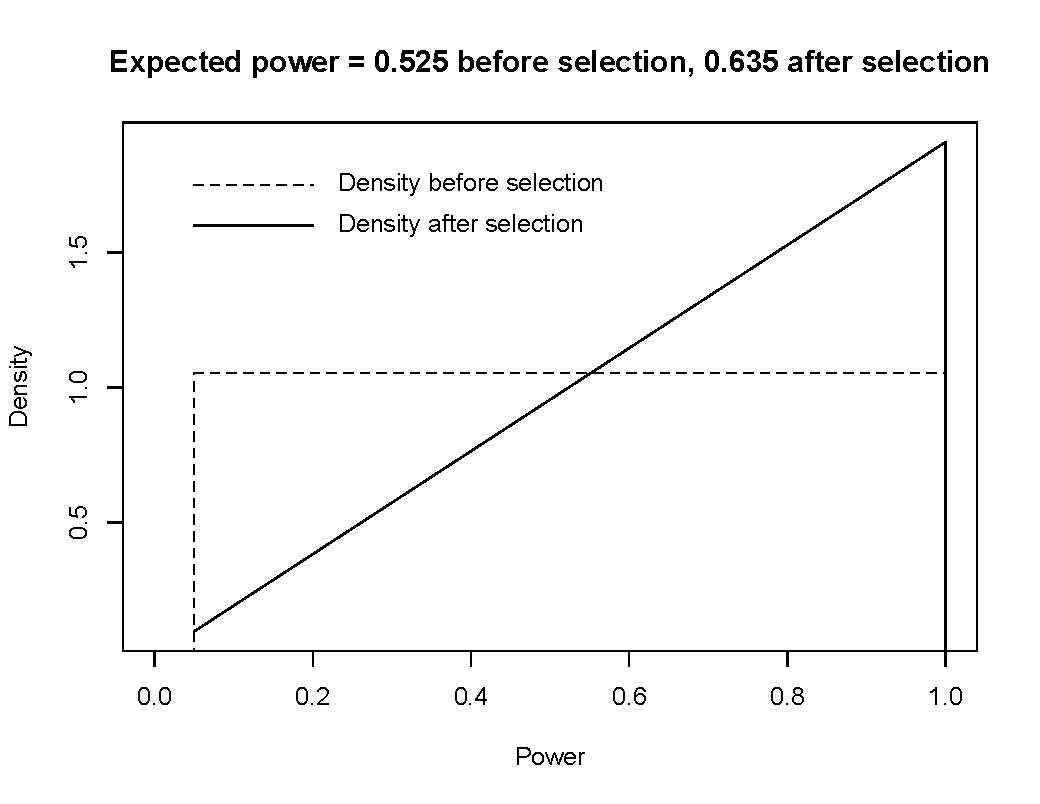
\includegraphics[width=3in]{pictures/density1} 
\label{pdfmult1} % Label after figure or numbering is wrong
\end{figure}
 In Figure~\ref{pdfmult2}, power before selection is less heterogeneous, and higher on average. Consequently, the distributions of power before selection and after selection are much more similar. In both cases, though, mean true power after selection for significance is higher.
\begin{figure}[h] 
\caption{Chi-squared distribution of power before selection}
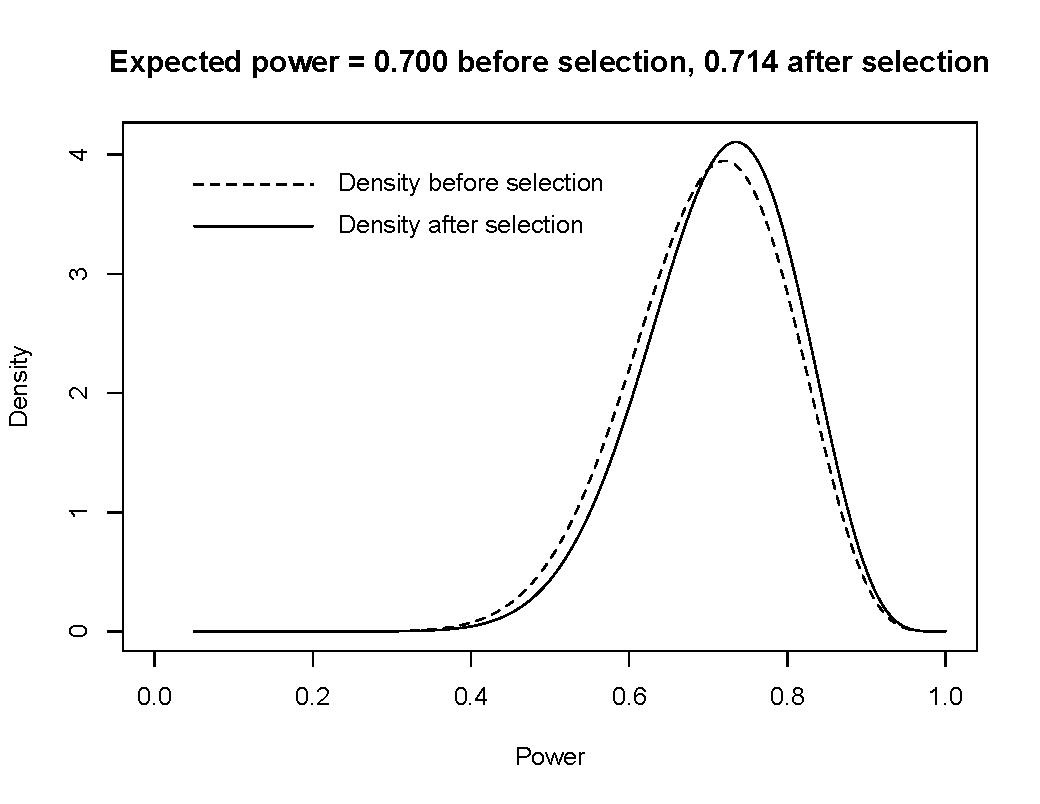
\includegraphics[width=3in]{pictures/density2}
\label{pdfmult2} % Label after figure or numbering is wrong
\end{figure}

In the Appendix, Principle~\ref{pdf} is used to derive the remaining principles. The next Principle shows how mean power after selection is related to mean power before selection. In the simulations, it is used to choose the parameters of distributions before selection so that expected power after selection will have some desired value. 
Finding exactly the right values by trial and error is difficult.
\begin{princ} \label{meansquaredovermean}
Population mean power after selection for significance equals the population mean of squared power before selection, divided by the population mean of power before selection.  
\end{princ}
It is also possible to go back from power after selection to mean power before selection, again without knowing the full distributions. In Principle~\ref{recip}, the reciprocal of power refers to one divided by the power value. Naturally this quantity has a population mean.
\begin{princ} \label{recip}
Population mean power before selection equals one divided by the population mean of the reciprocal of power after selection.
\end{princ}
Although we do not pursue the topic in this paper, Principle~\ref{recip} opens the door to estimating mean power before selection (the typicl ``success rate" in a field) using only significant results.

Selection for significance is often called ``publication bias" \parencite{Sterling1959, SterlingEtAl1995}, and it has indisputable drawbacks. However, it does increase average power because tests with higher power are more likely to be selected. Principle~\ref{increase} quantifies the increase.
\begin{princ} \label{increase}
The increase in population mean power due to selection for significance equals the population variance of power before selection divided by the population mean of power before selection.
\end{princ}
Because variances cannot be negative, population mean power after selection for significance is always greater than or equal to population mean power before selection, with equality occurring only in the homogeneous case where the population variance of power before selection is equal to zero. The greatest increases in mean power will occur when the distribution of power before selection is heterogeneous, and average power is low.

Since power arises from the combination of sample size with effect size, selection for significance affects both. This last Principle shows how selection affects the joint probability distribution of sample size and effect size. The similarity to Principle~\ref{pdf} is remarkable.

\begin{princ} \label{jointNes}
The effect of selection for significance is to multiply the joint distribution of sample size and effect size before selection by power for that sample size and effect size, divided by population mean power before selection.
\end{princ}

Principle~\ref{jointNes} implies that if sample size and effect size are independent before selection they cannot be independent after selection, and vice versa. In simulations, it allows the distribution of sample size before selection to be constructed so that selection for significance produces a sample size distribution that matches observed data. An observed distribution of sample sizes after selection may imply a large proportion of studies before selection with very small sample sizes. Most of these small-sample studies are filtered out by the selection process --- in theory. 

\section{Estimation Methods} \label{METHODS}

In this section, we describe four methods for estimating population mean power under conditions of heterogeneity, after selection for statistical significance. 

\subsection{P-curve 2.1 and p-uniform estimation of mean power} \label{PCU}
The original p-curve~2.0 \parencite{SimonsohnEtAl2014b} and p-uniform \parencite{vanAssenEtAl2014} methods are  designed for estimating effect sizes in meta-analyses where there is a single fixed effect size, but possibly varying sample sizes. We adapted them slightly to produce estimates of mean power, again for the setting of heterogeneity in sample size but not effect size. As stated earlier, we refer to our adaptation of p-curve as p-curve~2.1.

Both p-uniform and p-curve~2.1 are based on the idea that $p$-values are uniformly distributed when the null hypothesis is true. Originally, the test statistics were used to test the null hypothesis that the effect size is zero, and they all rejected that null hypothesis.  Now the set of significant test statistics is used to test a \emph{modified} null hypothesis that the effect size equals some specified non-zero value. If the modified null hypotheses were true, the resulting $p$-values would again have a uniform distribution. To find the best fitting effect size for a set of observed test statistics, p-curve~2.1 and p-uniform compute p-values for various effect sizes and chose the effect size that yields the best approximation of a uniform distribution. % The main difference between p-curve~2.1 and p-uniform is the criterion used to pick the best fitting effect size. % Ui says later. 

If the modified null hypothesis that effect size = \texttt{es} is true, the cumulative distribution function of the test statistic is the conditional probability
\begin{eqnarray*}
    F_0(t) & = & Pr\{T \leq t | T > c\} \\
    & = & \frac{\R{p(}t\R{,ncp}\R{)}-\R{p(}c\R{,ncp}\R{)}}{1-\R{p(}c\R{,ncp}\R{)}} \\
    & = & \frac{\R{p(}t\R{,}f_1(n)\cdot f_2(\R{es})\R{)}-\R{p(}c\R{,}f_1(n)\cdot f_2(\R{es})\R{)}}
               {1-\R{p(}c\R{,}f_1(n_i)\cdot f_2(\R{es})\R{)}} ,
\end{eqnarray*}
using $\R{ncp} = f_1(n)\cdot f_2(\R{es})$ as given in Equation~\ref{ncpmult}. The corresponding modified $p$-value 
%(which Simonsohn et al. would call the $pp$-value) 
is 
\begin{displaymath}
    1-F_0(T) = \frac{1-\R{p(}T\R{,}f_1(n)\cdot f_2(\R{es})\R{)}}
               {1-\R{p(}c\R{,}f_1(n)\cdot f_2(\R{es})\R{)}}.
\end{displaymath} 
Note that since the sample sizes of the tests may differ, the symbols \texttt{p}, $n$ and $c$ as well as $T$ may %refer to different things 
have different referents for $j=1, \ldots, k$ test statistics. The subscript $j$ has been omitted to reduce notational clutter.

If the modified null hypothesis were true, the modified $p$-values would have a uniform distribution. Both p-curve~2.1 and p-uniform choose as estimated effect size the value of $\R{es}$ that makes the modified $p$-values most nearly uniform. They differ only in the criterion for deciding when uniformity has been reached. 

P-curve~2.1 is based on a Kolmogorov-Smirnov test for departure from a uniform distribution, choosing the $\R{es}$ value yielding the smallest value of the test statistic. $P$-uniform is based on a different criterion. Denoting by $P_j$ the modified $p$-value associated with test $j$, calculate $Y = -\sum_{j=1}^k\ln({P_j})$, where $\ln$ is the natural logarithm. If the $P_j$ values were uniformly distributed, $Y$ would have a Gamma distribution with expected value $k$, the number of tests. The P-uniform estimate is the modified null hypothesis effect size $\R{es}$ that makes $Y$ equal to $k$, its expected value under uniformity.

These technologies are designed for heterogeneity in sample size only, and assume a common effect size for all the tests. Given an estimate $\widehat{\R{es}}$ of the common effect size, estimated power for each test is solely determined by sample size. Using Expression~\ref{powereq}, the estimated power of test $j$ is $1-\R{p(}c_j\R{,}f_1(n_j)\cdot f_2(\widehat{\R{es}})\R{)}$. Population mean power can then be estimated by averaging the $k$ power estimates. This natural way of estimating mean power is merely implicit in the papers by van Assen et al.~(2014) and Simonsohn et al.~(2014b). 

\subsection{Maximum likelihood}\label{MLE} 

The mechanism for data generation would be fully determined if the joint distribution of sample size and effect size were known. Because sample size values are directly observable, we escape from assuming a distribution for them by conducting the analysis conditionally upon their values. This is deliberately similar to the way that independent variable values are treated as fixed constants in the theory of multiple regression. To take selection for significance into account, the likelihood function for this problem is a product of $k$ conditional densities; each term is the conditional density of the test statistic $T_j$, given $N_j=n_j$ and $T_j>c_j$, the critical value.

\paragraph{Likelihood function}
For simplicity, assume that the sample size and effect size before selection for significance are independent, an assumption that does no harm when it is violated in the simulations. Suppose that the distribution of effect size before selection is continuous with probability density $g_\theta(\R{es})$. This notation indicates that the distribution of effect size depends on an unknown parameter or parameter vector $\theta$. In the appendix, it is shown that the likelihood function (a function of $\theta$) is a product of $k$ terms of the form
\begin{equation}\label{likehetero}
    \frac{\int_0^\infty\R{d(}t_j\R{,}f_1(n_j) \cdot f_2(\R{es})\R{)}g_\theta(\R{es}) \, d\R{es}}  {\int_0^\infty\left[1-\R{p(}c_j\R{,}f_1(n_j) \cdot f_2(\R{es})\R{)}\right]g_\theta(\R{es}) \, d\R{es}},
\end{equation}
where the integrals denote areas under curves that can be computed with R's \texttt{integrate} function. The maximum likelihood estimate, denoted by $\widehat{\theta}$ is the value of $\theta$ for which the value of the product is highest. Typically $\widehat{\theta}$ is a single number or a pair of numbers located by a numerical search.

An estimate of population mean power is produced by averaging estimated power for the $k$ significance tests. 
% Applying Principle~\ref{meansquaredovermean} to the conditional distribution of power given sample size and estimating $\widehat{\theta}$ with $\widehat{\theta}$, the terms to be averaged are
As shown in the appendix, the terms to be averaged are
\begin{equation}\label{heteromle}
\frac{\int_0^\infty\left[1-\R{p(}c_j\R{,}f_1(n_j) \cdot f_2(\R{es})\R{)}\right]^2
      g_{\widehat{\theta}}(\R{es}) \, d\R{es}} 
     {\int_0^\infty\left[1-\R{p(}c_j\R{,}f_1(n_j) \cdot f_2(\R{es})\R{)}\right]
      g_{\widehat{\theta}}(\R{es}) \, d\R{es}}.
\end{equation}

% Comments: In EdBehStat2 and earlier, I have an intense and lengthy calculation to get the last expression.  
% In the calculation of likelihood, everything is conditional on T>c, because we can only see significant results, even the density of effect size. I've made the estimation conditional on N=n too, as in regression. Then when we average estimated power values to get estimated mean power, we are really estimating the distribution of N|T>c by its empirical distribution function, and integrating with respect to that. This is fairly clear in the appendix.

\subsection{$Z$-curve}\label{ZCURVE}      

$Z$-curve follows a traditional meta-analyses that converts $p$-values into $Z$-scores as a common metric to integrate results from different original studies \parencite{StoufferEtAl1949, Rosenthal1979}. The use of $Z$-scores as a common metric makes it possible to fit a single function to $p$-values arising from widely different statistical methods and tests. The method is based on the simplicity and tractability of power analysis for the one-tailed $Z$-test, in which the distribution of the test statistic under the alternative hypothesis is just a standard normal shifted by a fixed quantity that plays the role of a non-centrality parameter, and will be denoted by $m$. Input to the $Z$-curve is a sample of $p$-values, all less than $\alpha=0.05$. These $p$-values are processed in several steps to produce an estimate.
\begin{enumerate}
     \item \emph{Convert $p$-values to $Z$-scores}. The first step is to imagine, for simplicity, that all the $p$-values arose from two-tailed $Z$-tests in which results were in the predicted direction. This is equivalent to an upper-tailed $Z$-test with significance level $\alpha/2 = 0.025$. The conversion to $Z$-scores \parencite{StoufferEtAl1949} consists of finding the test statistic $Z$ that would have produced that $p$-value. The formula is
\begin{equation} \label{Zformula}
    Z = \R{qnorm(}1-p/2\R{)} .
\end{equation}
     \item \emph{Set aside $Z>6$}. We assume that $p$-values in this range come from tests with power essentially equal to one. To avoid numerical problems arising from $p\approx 0$, we set them aside for now and bring them back in the final step.
     \item \label{zfit} \emph{Fit a finite mixture model}. Before selecting  for significance and setting aside values above six, the distribution of the test statistic $Z$ given a particular non-centrality parameter value $m$ is normal with mean $m$. Afterwards, it is a normal distribution truncated on the left at the critical value $c$ (usually 1.96) truncated on the right at 6, and re-scaled to have area one under the curve. 

Because of heterogeneity in sample size and effect size, the full distribution of $Z$ is an average of truncated normals, with potentially a different value of $m$ for each member of the population. As a simplification, heterogeneity in the distribution of $Z$ is represented as a finite mixture with $r$ components. The model is equivalent to the following two-stage sampling plan. First, select a non-centrality parameter $m$ from $m_1, \ldots, m_r$ according to the respective probabilities $w_1, \ldots, w_r$. Then generate $Z$ from a normal distribution with mean $m$ and standard deviation one. Finally, truncate and re-scale. 

Under this approximate model, the probability density function of the test statistic after selection for significance is 
\begin{equation} \label{Zmixture}
    f(z) = \sum_{j=1}^r w_j \, \frac{\R{dnorm(}z-m_j\R{)} }
            { \R{pnorm(}6-m_j\R{)} - \R{pnorm(}c-m_j\R{)} }.
\end{equation} 
% Mixing first and then truncating would yield estimates of w_j before selection. Oh really?

The finite mixture model is only an approximation. If the true probability density function of $Z$ given significance were known, the approximation could be optimized by choosing $w_1, \ldots, w_r$ and $m_1, \ldots, m_r$ to bring (\ref{Zmixture}) as close to the true density as possible. Since the true density is unknown, we use a kernel density estimate \parencite{Silverman1986} as implemented in R's \texttt{density} function, with the default settings.   

Specifically, the fitting step proceeds as follows. First, obtain the kernel density estimate based on the sample of significant $Z$ values, re-scaling it so that the area under the curve between 1.96 and 6 equals one. Call this the \emph{conditional density estimate}. Next, calculate the conditional density estimate at a set of equally spaced points ranging from 2 to 6. Then, numerically choose $w_j$ and $m_j$ values so as to minimize the sum of absolute differences between the conditional density estimate and~(\ref{Zmixture}).  

     \item \emph{Estimate mean power for $Z<6$}. The estimate of rejection probability upon replication for $Z<6$ is the area under the curve above the critical value, with weights and non-centrality values from the curve fitting step. The estimate is
\begin{equation} \label{Zestimate1}
    \ell = \sum_{j=1}^r \widehat{w}_j (1-\R{pnorm(}c-\widehat{m}_j\R{)}),
\end{equation}
where $\widehat{w}_1, \ldots, \widehat{w}_r$ and $\widehat{m}_1, \ldots, \widehat{m}_r$ are the values located in Step~\ref{zfit}. Note that while the input data are censored both on the left and right as represented in Forumula~\ref{Zmixture}, there is no truncation in Formula~\ref{Zestimate1} because it represets the distribution of $Z$ upon replication.
     \item \emph{Re-weight using $Z>6$}. Let $q$ denote the proportion of the original set of $Z$ statistics with $Z>6$. Again, we assume that the probability of significance for those tests is essentially one. Bringing this in as one more component of the mixture estimate, the final estimate of the probability of rejecting the null hypothesis for exact replication of a randomly selected test is  
\begin{eqnarray} \label{zcurveestimate}
    Z_{est} &=& (1-q) \, \ell + q \cdot 1 \\ \nonumber
      &=& q + (1-q)\sum_{j=1}^r \widehat{w}_j (1-\R{pnorm(}c-\widehat{m}_j\R{)})
\end{eqnarray}

\end{enumerate}
By Principle~\ref{doubleex}, this is also an estimate of population true mean power after selection.

\section{Simulations} \label{SIMS}
The simulations reported here were carried out using the R programming environment (R Core Team, 2012) distributing the computation among 70 quad core Apple iMac computers. The R code is available in the supplementary materials, at \\
{\small
\href{http://www.utstat.toronto.edu/~brunner/zcurve2018}
     {\texttt{http://www.utstat.toronto.edu/$\sim$brunner/zcurve2018}}. 
} % End size     
In the simulations, the four estimation methods (p-curve~2.1, p-uniform, maximum likelihood and z-curve) were applied to samples of significant chi-squared or $F$ statistics, all with $p < 0.05$. This covers most cases of interest, since $t$ statistics may be squared to yield $F$ statistics, while $Z$ may be squared to yield chi-squared with one degree of freedom. 

\subsection{Heterogeneity in Sample Size Only: Effect size fixed} \label{HETERON}
Sample sizes after selection for significance were randomly generated from a Poisson distribution with mean 86, so that they were approximately normal, with population mean 86 and population standard deviation 9.3. Population mean power, number of test statistics on which the estimates were based, type of test (chi-squared or $F$) and (numerator) degrees of freedom were varied in a complete factorial design. Within each combination, we generated 10,000 samples of significant test statistics and applied the four estimation methods to each sample. In these simulations, it was not necessary to simulate test statistic values and then literally select those that were significant. A great deal of computation was saved by using the R~functions \texttt{rsigF} and \texttt{rsigCHI}, (available from the \href{http://www.utstat.toronto.edu/~brunner/zcurve2018} {supplementary materials}) to simulate directly from the distribution of the test statistic after selection. A description of the simulation method and a  proof of its correctness are given in the appendix.

Effect sizes were selected to yield population mean power values after selection of 0.05, 0.25, 0.50 or 0.75. For $F$-tests, we used \citeauthor{Cohen1988}'s (\citeyear[][p.~275]{Cohen1988}) effect size metric $\mathbf{f}$. For chi-squared tests, we used Cohen's $\mathbf{w}$ \parencite[][p.~216]{Cohen1988}. The number of test statistics $k$ on which estimates were based was 15, 25, 50, 100 or 250. Numerator degrees of freedom (just degrees of freedom for the chi-squared tests) were one, three or five. Because the pattern of results was similar for $F$ and chi-squared tests and for different degrees of freedom, we give details for $F$-tests with one numerator degree of freedom; preliminary data mining of the psychological literature suggests that this is the case most frequently encountered in practice. Full results are given in the \href{http://www.utstat.toronto.edu/~brunner/zcurve2018} {supplementary materials}.

\paragraph{Average performance} Table \ref{heteroNmean} shows mean estimated population mean power after selection, based on 10,000 simulations in each condition. Standard deviations are given in the \href{http://www.utstat.toronto.edu/~brunner/zcurve2018} {supplementary materials}. Differences between the estimates and the true values represent bias in estimation. We conclude that all methods performed fairly well, with z-curve showing a bit more bias than the other methods. The z-curve estimates were also more variable. This is understandable, since the other methods directly use information about sample size, and z-curve does not.

\begin{table}
\caption{Average estimated population mean power for heterogeneity in sample size only: $F$-tests with numerator $df=1$}
{\small
\begin{center}
\begin{tabular}{lrrrrr}  \hline
      & \multicolumn{5}{c}{Number of Tests}\\ 
      &  15 & 25 & 50 & 100 & 250 \\ \hline
\multicolumn{6}{l}{\textbf{Population Mean Power = 0.05}} \\ \hline
P-curve~2.1   & 0.083 & 0.073 & 0.064 & 0.059 & 0.055  \\
P-uniform & 0.076 & 0.067 & 0.061 & 0.058 & 0.054  \\
MaxLike   & 0.076 & 0.067 & 0.061 & 0.057 & 0.054  \\
Z-curve   & 0.086 & 0.071 & 0.058 & 0.049 & 0.040  \\ \hline
\multicolumn{6}{l}{\textbf{Population Mean Power = 0.25}} \\ \hline
P-curve~2.1   & 0.269 & 0.261 & 0.256 & 0.253 & 0.251 \\
P-uniform & 0.256 & 0.253 & 0.252 & 0.251 & 0.251 \\
MaxLike   & 0.260 & 0.255 & 0.253 & 0.251 & 0.251 \\
Z-curve   & 0.314 & 0.305 & 0.293 & 0.280 & 0.268 \\ \hline
\multicolumn{6}{l}{\textbf{Population Mean Power = 0.50}} \\ \hline
P-curve~2.1   & 0.484 & 0.491 & 0.496 & 0.497 & 0.499 \\
P-uniform & 0.473 & 0.485 & 0.493 & 0.496 & 0.499  \\
MaxLike   & 0.479 & 0.489 & 0.495 & 0.497 & 0.499 \\
Z-curve   & 0.513 & 0.516 & 0.513 & 0.508 & 0.502 \\ \hline
\multicolumn{6}{l}{\textbf{Population Mean Power = 0.75}} \\ \hline
P-curve~2.1   & 0.728 & 0.736 & 0.742 & 0.747 & 0.749 \\
Puniform & 0.721 & 0.732 & 0.740 & 0.746 & 0.748  \\
MaxLike  & 0.728 & 0.736 & 0.742 & 0.747 & 0.749 \\
Zcurve   & 0.704 & 0.712 & 0.717 & 0.723 & 0.728 \\ \hline
\end{tabular}
\end{center}
} % End size
\label{heteroNmean}  % Label must come after the table or numbering is wrong. But see below.
\end{table}

\paragraph{Absolute error of estimation}
It is desirable for average estimates to be close to the true values, but still positive and negative errors may cancel. More interesting is how close the estimate is on average to the true value being estimated. Table \ref{heteroNabserrF} shows mean absolute error of estimation for $F$-tests with one numerator degree of freedom; full results are givn in the \href{http://www.utstat.toronto.edu/~brunner/zcurve2018} {supplementary materials}. As expected, all the methods become more accurate with larger numbers of tests. Though the differences are fairly small, Z-curve is least accurate when mean power is low, and most accurate when mean power is high. Maximum likelihood has a slight edge over the other methods under most circumstances, except that z-curve sometimes does better when population mean power is moderate to high and the estimates are based on a small number of tests.

\begin{table} % [!h]
\caption{Mean absolute error of estimation for heterogeneity in sample size only: $F$-tests with numerator $df=1$}
{\small
\begin{center}
\begin{tabular}{lrrrrr}  \hline
      & \multicolumn{5}{c}{Number of Tests} \\
      &  15 & 25 & 50 & 100 & 250 \\ \hline
      \multicolumn{6}{l}{\textbf{Population Mean Power = 0.05}} \\ \hline
P-curve~2.1    & 3.32  & 2.25  & 1.41  & 0.93  & 0.52 \\
P-uniform  & 2.57  & 1.75  & 1.11  & 0.76  & 0.43 \\
MaxLike    & 2.59  & 1.74  & 1.09  & 0.73  & 0.39 \\
Z-curve    & 6.53  & 4.90  & 3.38  & 2.44  & 1.79 \\ \hline
\multicolumn{6}{l}{\textbf{Population Mean Power = 0.25}} \\ \hline
P-curve~2.1   & 12.94 & 10.49  & 7.69  & 5.53  & 3.64 \\
P-uniform & 12.11  & 9.87  & 7.17  & 5.18  & 3.38 \\
MaxLike   & 12.07  & 9.76  & 7.05  & 5.10  & 3.32 \\
Z-curve   & 13.55 & 11.09  & 8.21  & 5.96  & 3.87 \\ \hline
\multicolumn{6}{l}{\textbf{Population Mean Power = 0.50}} \\ \hline
P-curve~2.1   & 14.32 & 11.20  & 8.14  & 5.80  & 3.67 \\
P-uniform & 13.93 & 10.68  & 7.80  & 5.56  & 3.51 \\
MaxLike   & 13.61 & 10.41  & 7.60  & 5.39  & 3.41 \\
Z-curve   & 12.42 &  9.91  & 7.44  & 5.48  & 3.59 \\ \hline
\multicolumn{6}{l}{\textbf{Population Mean Power = 0.75}} \\ \hline
P-curve~2.1    & 9.77  & 7.59  & 5.38  & 3.72  & 2.35 \\
P-uniform  & 9.79  & 7.59  & 5.34  & 3.71  & 2.32 \\
MaxLike    & 9.33  & 7.23  & 5.11  & 3.53  & 2.21 \\
Z-curve    & 8.34  & 6.96  & 5.56  & 4.30  & 3.13 \\ \hline
\end{tabular}
\end{center}
} % End size
\label{heteroNabserrF}  % Label must come after the table or numbering is wrong. 
\end{table}

\paragraph{Testing differences in accuracy} Because results like the ones in in Table~\ref{heteroNabserrF} are based on random number generation, some of the apparent differences could be due to chance. Thus we find ourselves applying statistical tests to an investigation of statistical tests.  Within each of the 20 combinations of mean true power and number of tests, there are six potential pairwise comparisons of mean absolute error. These comparisons were carried out using large-sample two-sided matched Z-tests with a Bonferroni correction, yielding a joint 0.001 significance level for the 120 tests.  

Tables \ref{heteroNchisqContest} and \ref{heteroNftestContest} show the number of times that the row method was significantly more accurate than the column method by this stringent criterion. For example, for chi-squared tests with one degree of freedom, p-curve~2.1 was significantly more accurate than z-curve 14 times, while z-curve was significantly more accurate than p-curve~2.1 for 5 treatment combinations. 

Tables \ref{heteroNchisqContest} and \ref{heteroNftestContest} each have three sub-tables, one for each degrees of freedom value. Note that the Bonferroni correction was applied separately to each sub-table. In all, Tables \ref{heteroNchisqContest} and \ref{heteroNftestContest} summarize the results of 720 tests. Full details are given in the \href{http://www.utstat.toronto.edu/~brunner/zcurve2018} {supplementary materials}. 

\begin{table} % [h]
\caption{Number of times row method is significantly more accurate than column method: Chi-squared tests, heterogeneity in sample size only}
{\small
\begin{center}
\begin{tabular}{l c ccccc }  \hline
\multicolumn{7}{c}{$df=1$} \\ \hline
& &       PC & PU & ML & ZC & Total  \\
P-curve~2.1   & (PC)   &  0    &    0   &    0  &   14 & 14   \\
P-uniform & (PU)   & 15    &    0   &    0  &   14 & 29   \\
MaxLike   & (ML)   & 20    &   16   &    0  &   16 & 52   \\
Z-curve   & (ZC)   &  5    &    4   &    3  &    0 & 12 \\ \hline
\multicolumn{7}{c}{$df=3$} \\ \hline
P-curve~2.1   & (PC)   &  0    &    0   &    0  &   15 & 15  \\
P-uniform & (PU)   & 16    &    0   &    0  &   15 & 31   \\
MaxLike   & (ML)   & 20    &   15   &    0  &   16 & 51  \\
Z-curve   & (ZC)   &  5    &    2   &    2  &    0 &  9 \\ \hline
\multicolumn{7}{c}{$df=5$} \\ \hline
P-curve~2.1   & (PC)  &   0    &    0   &    0  &   15 & 15   \\
P-uniform & (PU)  &   15   &    0   &    1  &   16 & 32  \\
MaxLike   & (ML)  &   20   &   15   &    0  &   17 & 52  \\
Z-curve   & (ZC)  &    3   &    2   &    2  &    0 &  7   \\ \hline
\end{tabular}
\end{center}
} % End size
\label{heteroNchisqContest}  % Label must come after the table or numbering is wrong. 
\end{table}
% 

\begin{table} % [h]
\caption{Number of times row method is significantly more accurate than column method: $F$-tests, heterogeneity in sample size only}
{\small
\begin{center}
\begin{tabular}{l c ccccc }  \hline
\multicolumn{7}{c}{Numerator $df=1$} \\ \hline
& &       PC & PU & ML & ZC & Total  \\
P-curve~2.1   & (PC)   &  0    &    0   &    0  &   13 & 13  \\
P-uniform & (PU)   & 15    &    0   &    0  &   13 & 28  \\
MaxLike   & (ML)   & 20    &   17   &    0  &   14 & 51  \\
Z-curve   & (ZC)   &  7    &    5   &    4  &    0 & 16  \\ \hline
\multicolumn{7}{c}{Numerator $df=3$} \\ \hline
P-curve~2.1   & (PC)   &  0    &    0   &    0  &   13 & 13  \\
P-uniform & (PU)   & 15    &    0   &    0  &   14 & 29  \\
MaxLike   & (ML)   & 20    &   16   &    0  &   15 & 51  \\
Z-curve   & (ZC)   &  6    &    4   &    3  &    0 & 13  \\ \hline
\multicolumn{7}{c}{Numerator $df=5$} \\ \hline
P-curve~2.1   & (PC)  &   0    &    0   &    0  &   13 & 13  \\
P-uniform & (PU)  &   14   &    0   &    0  &   14 & 28  \\
MaxLike   & (ML)  &   20   &   16   &    0  &   15 & 51  \\
Z-curve   & (ZC)  &    6   &    4   &    3  &    0 & 13  \\ \hline
\end{tabular}
\end{center}
} % End size
\label{heteroNftestContest}  % Label must come after the table or numbering is wrong. 
\end{table}

% \noindent
In each sub-table of Tables \ref{heteroNchisqContest} and \ref{heteroNftestContest}, the most accurate method overall is maximum likelihood, followed by p-uniform. When maximum likelihood lost a comparison it was usually to z-curve -- especially when mean power was moderate to high and the number of tests on which the estimates were based was low. P-curve~2.1 and z-curve were least accurate overall, with p-curve~2.1 perhaps having a slight edge for chi-squared tests with larger degrees of freedom.

As one would expect from the large-sample theory of maximum likelihood estimation 
\parencite[][Ch.~6]{LehmanCasella1998}, maximum likelihood performed particularly well when estimates were based on a large number of tests. It is important to recognize, however, the the differences in average estimation error are fairly small. We conclude that although maximum likelihood performs best, all the methods yield reasonable estimates when effect sizes are homogeneous. 


\subsection{Heterogeneity in Both Sample Size and Effect Size} \label{HETERONES}

To model heterogeneity in effect size, we let effect size before selection vary according to a gamma distribution \parencite{JohnsonEtAl1995}, a flexible continuous distribution taking positive values. Sample size before selection remained Poisson distributed with a population mean of 86. For convenience, sample size and effect size were independent before selection for significance. Maximum likelihood correctly assumed a gamma distribution for effect size, and the likelihood search was over the two parameters of the gamma distribution. The other three methods were not modified in any way. P-curve~2.1 and p-uniform continued to assume a fixed effect size, and z-curve continued to assume heterogeneity in the non-centrality parameter without distinguishing between heterogeneity in sample size and heterogeneity in effect size.

We carried out a simulation experiment like the one in Section~\ref{HETERON},
%for heterogeneity in sample size only, 
with one additional factor: amount of heterogeneity in effect size, as represented by the standard deviation of the effect size distribution. The factors were true population mean power (0.25, 0.50 or 0.75), standard deviation of effect size after selection (0.10, 0.20 or 0.30), number of test statistics upon which estimates of mean power are based ($k=$100, 250, 500, 1,000 or 2,000), type of test ($F$ or chi-squared), and experimental degrees of freedom (1, 3 or 5). Within each cell of the design, ten thousand significant chi-squared test statistics were randomly generated, and population mean power was estimated using all four methods. For brevity, we present results for $F$-tests with numerator $df=1$. Full results are given in the \href{http://www.utstat.toronto.edu/~brunner/zcurve2018} {supplementary materials}. 

When there is heterogeneity in effect size, maximum likelihood is computationally demanding. The areas under many curves must be calculated numerically; see Expression~\ref{likehetero}. Using R's \texttt{integrate} function, the calculation involves fitting a histogram to each curve and then adding the areas of the bars. It is slow, and some of the curves are very skewed and razor thin. Numerical accuracy is an issue, especially for ratios of areas when the denominators are very small. In addition, the likelihood function has many local maxima, and it is necessary to try more than one starting value to have a hope of locating the global maximum. In our simulations, we used three random starting points. More would have been better, but the computational burden was too great for a simulation study. As a result, we consider the performance of maximum likelihood to be somewhat under-stated. Note that speed would not be a serious issue in applications to real data, but here we are simulating 2,700,000 meta-analyses for this one section alone. 


\paragraph{Average performance} Table~\ref{heteromean} shows estimated population mean power as a function of true population mean power and the standard deviation of effect size size. Differences between the average estimates and population mean values represent bias in estimation. The averages are mean estimates over 10,000 simulated samples of test statistics. In this table the estimates were based on $k=1,000$ test statistics, and good accuracy may be anticipated. P-uniform broke down completely for higher values of heterogeneity in effect size, with most estimates close to one regardless of the true value.  For moderate to high mean power,  p-curve~2.1 also produced an over-estimate on average, with the problem becoming most severe when mean power and heterogeneity in effect size were both high. Maximum likelihood and z-curve performed much better. 

\begin{table}[h]
\caption{Average estimated power for heterogeneity in sample size and effect size based on $k=1,000$ $F$-tests with numerator $df=1$}
{\small
\begin{center}
\begin{tabular}{lccc c lccc}  \hline
      & \multicolumn{3}{c}{\emph{SD} of Effect Size} \\ 
          &  0.1  &  0.2  &  0.3    \\ \hline
\multicolumn{4}{l}{\textbf{Population Mean Power = 0.25}} \\ \hline
P-curve~2.1   & 0.225 & 0.272 & 0.320    \\
P-uniform & 0.294 & 0.694 & 0.949    \\
MaxLike   & 0.230 & 0.269 & 0.283    \\
Z-curve   & 0.233 & 0.225 & 0.226    \\ \hline
\multicolumn{4}{l}{\textbf{Population Mean Power = 0.50}} \\ \hline
P-curve~2.1   & 0.549 & 0.679 & 0.757    \\
P-uniform & 0.602 & 0.913 & 0.995   \\
MaxLike   & 0.501 & 0.502 & 0.506    \\
Z-curve   & 0.504 & 0.492 & 0.487   \\ \hline
\multicolumn{4}{l}{\textbf{Population Mean Power = 0.75}} \\ \hline
P-curve~2.1   & 0.824 & 0.928 & 0.962   \\
P-uniform & 0.861 & 0.992 & 1.000    \\
MaxLike   & 0.752 & 0.750 & 0.750    \\
Z-curve   & 0.746 & 0.755 & 0.760   \\ \hline
\end{tabular}
\end{center}
} % End size
\label{heteromean}  % Label must come after the table or numbering is wrong. 
\end{table}

\paragraph{Absolute error of estimation}
Table~\ref{heteroabserr} shows mean absolute error of estimation. It confirms the inaccuracy of p-uniform under heterogeneity in effect size, and suggests that p-curve~2.1 may be competitive with maximum likelihood and z-curve when heterogeneity and true mean power are both low. Otherwise, p-curve~2.1 can severely over-estimate population mean power. 

\begin{table}[h]
\caption{Mean absolute error of estimation in percentage points, for heterogeneity in sample size and gamma effect size based on $k=1,000$ $F$-tests with numerator $df=1$}
{\small
\begin{center}
\begin{tabular}{lccc}  \hline
      & \multicolumn{3}{c}{\emph{SD} of Effect size} \\
           &  0.1   &  0.2    & 0.3  \\ \hline
\multicolumn{4}{l}{\textbf{Population Mean Power = 0.25}} \\ \hline
P-curve~2.1    & ~2.87  & ~3.16  & ~7.08   \\
P-uniform  & ~4.50  & 44.38  & 69.90   \\
MaxLike    & ~3.55  & ~2.06  & ~3.34   \\
Z-curve    & ~2.59  & ~3.08  & ~2.90   \\ \hline
\multicolumn{4}{l}{\textbf{Population Mean Power = 0.50}} \\ \hline
P-curve~2.1    & ~4.93  & 17.86 & 25.70   \\
P-uniform  & 10.21  & 41.28 & 49.54   \\
MaxLike    & ~1.80  & ~1.49 & ~1.50   \\
Z-curve    & ~2.12  & ~2.19 & ~2.23   \\ \hline
\multicolumn{4}{l}{\textbf{Population Mean Power = 0.75}} \\ \hline
P-curve~2.1    & ~7.45  & 17.75 & 21.23   \\
P-uniform  & 11.08  & 24.17 & 24.99   \\
MaxLike    & ~1.42  & ~1.18 & ~1.16   \\
Z-curve    & ~1.69  & ~1.42 & ~1.55   \\ \hline
\end{tabular}
\end{center}
} % End size
\label{heteroabserr}  % Label must come after the table or numbering is wrong. 
\end{table}

\paragraph{Testing differences in accuracy} Table~\ref{heteroabserr} is a sub-table, giving results based on $k=1,000$ $F$-tests with numerator $df=1$. The full simulation study has 3 levels of population mean true power, 3 levels of the standard deviation of effect size (heterogeneity), and 5 levels of number of tests $k$. Within each of these 45 combinations, there are 6 pairwise comparisons of the 4 estimation methods. The resulting 270 matched $Z$-tests were protected with a Bonferroni correction at the joint 0.001 significance level. This correction was applied separately for $F$-tests and chi-squared tests. Table~\ref{heteroChisqContest} counts the wins for chi-squared tests, and Table~\ref{heteroFtestContest} counts the wins for $F$-tests. 

\begin{table} % [h]
\caption{Number of times row method is significantly more accurate than column method: Chi-squared tests, heterogeneity in sample size and gamma effect size}
{\small
\begin{center}
\begin{tabular}{l c ccccc }  \hline
\multicolumn{7}{c}{$df=1$} \\ \hline
& &       PC & PU & ML & ZC & Total  \\
P-curve~2.1   & (PC)   &  0       & 45      & 0     &  0  &  45  \\
P-uniform & (PU)   &  0       &  0      & 0     &  0  &   0  \\
MaxLike   & (ML)   & 41       & 45      & 0     & 33  & 119  \\
Z-curve   & (ZC)   & 45       & 45      & 8     &  0  &  98  \\ \hline
\multicolumn{7}{c}{$df=3$} \\ \hline
P-curve~2.1   & (PC)   &  0       & 45      &  4    &  1  &  50  \\
P-uniform & (PU)   &  0       &  0      &  0    &  0  &   0  \\
MaxLike   & (ML)   & 40       & 44      &  0    & 34  & 118  \\
Z-curve   & (ZC)   & 40       & 45      &  7    &  0  &  92  \\ \hline
\multicolumn{7}{c}{$df=5$} \\ \hline
P-curve~2.1   & (PC)  &   0       & 45      &  5    &  4  &  54  \\
P-uniform & (PU)  &   0       &  0      &  0    &  0  &   0  \\
MaxLike   & (ML)  &   40      & 45      &  0    & 36  & 121  \\
Z-curve   & (ZC)  &   38      & 45      &  5    &  0  &  88  \\ \hline
\end{tabular}
\end{center}
} % End size
\label{heteroChisqContest}  % Label must come after the table or numbering is wrong. 
\end{table}
% 

\begin{table} % [h]
\caption{Number of times row method is significantly more accurate than column method: $F$-tests, heterogeneity in sample size and gamma effect size}
{\small
\begin{center}
\begin{tabular}{l c ccccc }  \hline
\multicolumn{7}{c}{Numerator $df=1$} \\ \hline
& &       PC & PU & ML & ZC & Total  \\
P-curve~2.1   & (PC)   &  0       & 45      & 4     &  0  &  49  \\
P-uniform & (PU)   &  0       &  0      & 0     &  0  &   0  \\
MaxLike   & (ML)   & 40       & 45      & 0     & 31  & 116  \\
Z-curve   & (ZC)   & 42       & 45      & 10    &  0  &  97  \\ \hline
\multicolumn{7}{c}{Numerator $df=3$} \\ \hline
P-curve~2.1   & (PC)   &  0       & 45      &  5    &  4  &  54  \\
P-uniform & (PU)   &  0       &  0      &  5    &  0  &   5  \\
MaxLike   & (ML)   & 40       & 40      &  0    & 34  & 114  \\
Z-curve   & (ZC)   & 39       & 45      &  7    &  0  &  91  \\ \hline
\multicolumn{7}{c}{Numerator $df=5$} \\ \hline
P-curve~2.1   & (PC)  &   0       & 45      &  5    &  6  &  56  \\
P-uniform & (PU)  &   0       &  0      &  5    &  1  &   6  \\
MaxLike   & (ML)  &   40      & 40      &  0    & 34  & 114  \\
Z-curve   & (ZC)  &   38      & 42      &  8    &  0  &  88  \\ \hline
\end{tabular}
\end{center}
} % End size
\label{heteroFtestContest}  % Label must come after the table or numbering is wrong. 
\end{table}

For all three $df$ values and all five values of $k$ (the number of significance tests on which the estimates were based), Table~\ref{heteroChisqContest} counts the wins for chi-squared tests, and Table~\ref{heteroFtestContest} counts the wins for $F$-tests. Maximum likelihood is clearly the best, followed by z-curve, p-curve~2.1 and p-uniform in that order. When other methods beat maximum likelihood, it was almost always when heterogeneity in effect size and population mean true power were both low. This is consistent with Table~\ref{heteromean}, in which maximum likelihood performs best when mean power is moderate to high. 

\subsection{Violating the Assumptions} \label{VIOLATION}

In the preceding simulation study, heterogeneity in effect size before selection was modeled by a gamma distribution, with effect size independent of sample size before selection. Maximum likelihood had a substantial and arguably unfair advantage, since it assumed exactly the correct distribution for effect size. Also, maximum likelihood unfairly ``knew" that sample size and effect size before selection were independent. It is well known that when its assumptions are correct, maximum likelihood is very accurate compared to other methods \parencite[][Ch.~18]{StuartOrd1999}. When its assumptions are incorrect, the performance of maximum likelihood must be assessed on a case-by-case basis.

To test the robustness of maximum likelihood to assumptions, we conducted a smaller-scale simulation limited to $F$-tests with numerator degrees of freedom equal to one. Maximum likelihood continued to assume a gamma distribution for effect size before selection, but the true distribution was beta; see \textcite{JohnsonEtAl1995} for full details about these distributions. Though the beta distribution covers the interval zero to one and thus lacks the long right tail of the gamma, still the maximum value of one is more than more than twice 
\citeauthor{Cohen1988}'s (\citeyear[][p.~287]{Cohen1988})
large effect size of $\mathbf{f}=0.4$. 

Maximum likelihood also continued to assume independence of sample size and effect size before selection. We used a Poisson regression to connect them, inducing varying population correlations between sample size and effect size. Negative correlations would be expected, because of some researchers doing power analyses to select sample size,  or otherwise having a sense of the sample sizes required for significance in their fields of study.

In our simulations, the variance of effect size after selection was fixed at 0.30, the high heterogeneity value in the preceding section. Sample size after selection was Poisson distributed with expected value $\exp(\beta_0+\beta_1\R{es})$. Mean effect size after selection and the parameters $\beta_0$ and $\beta_1$ were selected to achieve (a) Desired population mean power after selection, (b) Desired population correlation between effect size and sample size after selection, and (c) Population mean sample size after selection equal to 86 at the mean effect size. Details are given in the appendix.

Three values of population mean power (0.25, 0.50 and 0.75), five values of the number of test statistics  ($k=$ 100, 250, 500, 1000 and 2000) and five values of the correlation between sample size and effect size (0.0, -0.2, -0.4, -0., -0.8) were varied in a factorial design, with ten thousand sets of simulated $F$ statistics at each combination of values. All four estimation methods were applied to each simulated data set, with three random starting values for maximum likelihood. 

Table~\ref{betacorrmean} shows average estimated population mean power as a function of true population mean power and the standard deviation of effect size. 
\begin{table} %[h]
\caption{Average estimated power with beta effect size and sample size correlated with effect size: $k = 1,000$ $F$-tests with numerator $df=1$}
{\small
\begin{center}
\begin{tabular}{lrrrrr}  \hline
& \multicolumn{5}{c}{Correlation between $n$ and \texttt{es}} \\ 
& -0.8 & -0.6 & -0.4 & -0.2 & 0.0 \\ \hline
\multicolumn{6}{l}{\textbf{Population Mean Power = 0.25}} \\ \hline
P-curve~2.1   & 0.407  & 0.405  & 0.403  & 0.403  & 0.402  \\
P-uniform & 0.853  & 0.852  & 0.852  & 0.852  & 0.852  \\
MaxLike   & 0.302  & 0.301  & 0.300  & 0.300  & 0.300   \\
Z-curve   & 0.232  & 0.231  & 0.230  & 0.231  & 0.230  \\ \hline
\multicolumn{6}{l}{\textbf{Population Mean Power = 0.50}} \\ \hline
P-curve~2.1   & 0.839  & 0.840  & 0.841  & 0.841  & 0.841   \\
P-uniform & 0.906  & 0.906  & 0.906  & 0.906  & 0.906   \\
MaxLike   & 0.532  & 0.533  & 0.533  & 0.534  & 0.534   \\
Z-curve   & 0.493  & 0.494  & 0.495  & 0.495  & 0.495   \\ \hline
\multicolumn{6}{l}{\textbf{Population Mean Power = 0.75}} \\ \hline
Pcurve   & 0.990  & 0.991  & 0.992  & 0.992  & 0.992    \\
Puniform & 0.964  & 0.966  & 0.966  & 0.967  & 0.967     \\
MaxLike  & 0.826  & 0.832  & 0.836  & 0.838  & 0.840    \\
Zcurve   & 0.785  & 0.790  & 0.793  & 0.794  & 0.796    \\ \hline
\end{tabular}
\end{center}
} % End size
\label{betacorrmean}  % Label must come after the table or numbering is wrong. 
\end{table}
In this table, the estimates were based on $k=1,000$ test statistics. Maximum likelihood tends to overestimate power when true power is high or low but not as much when true power equals 0.5. Correlation between sample size and effect size does not appear to matter much. P-curve~2.1 and p-uniform produce estimates that are much too high on average. The bias of z-curve is lowest overall.

Table~\ref{betacorrabserr} shows mean absolute error of estimation when estimates are based on $k=1,000$ test statistics. It shows maximum likelihood to be consistently less accurate than z-curve, though not as bad as p-curve~2.1 and p-uniform. Correlation between sample size and effect size appears to have little effect. Table~\ref{betacorrabserr} shows the results only for $k=1,000$ test statistics, but results are very similar for the other values of $k$. Full details are given in the \href{http://www.utstat.toronto.edu/~brunner/zcurve2018} {supplementary materials}. 


\begin{table}[h]
\caption{Mean absolute error of estimation in percentage points, with beta effect size and sample size correlated with effect size: $k = 1,000$ $F$-tests with numerator $df=1$}
{\small
\begin{center}
\begin{tabular}{lrrrrr}  \hline
      & \multicolumn{5}{c}{Correlation between $n$ and \texttt{es}} \\
      &  -0.8 & -0.6 & -0.4 & -0.2 & 0.0 \\ \hline
\multicolumn{6}{l}{\textbf{Population Mean Power = 0.25}} \\ \hline
P-curve~2.1   & 15.67  & 15.49  & 15.33  & 15.30  & 15.24 \\
P-uniform & 60.26  & 60.24  & 60.23  & 60.22  & 60.22 \\
MaxLike   &  5.17  &  5.11  &  5.05  &  5.05  &  5.01 \\
Z-curve   &  2.37  &  2.41  &  2.47  &  2.48  &  2.50 \\ \hline
\multicolumn{6}{l}{\textbf{Population Mean Power = 0.50}} \\ \hline
P-curve~2.1   & 33.88  & 33.99  & 34.07  & 34.09  & 34.11 \\
P-uniform & 40.59  & 40.61  & 40.63  & 40.63  & 40.64 \\
MaxLike   &  3.25  &  3.34  &  3.42  &  3.43  &  3.46 \\
Z-curve   &  1.92  &  1.91  &  1.89  &  1.90  &  1.89 \\ \hline
\multicolumn{6}{l}{\textbf{Population Mean Power = 0.75}} \\ \hline
P-curve~2.1   & 24.04  & 24.13  & 24.18  & 24.21  & 24.24 \\
P-uniform & 21.43  & 21.56  & 21.63  & 21.67  & 21.72 \\
MaxLike   &  7.62  &  8.23  &  8.56  &  8.76  &  8.97 \\
Z-curve   &  3.51  &  4.01  &  4.27  &  4.43  &  4.59 \\ \hline
\end{tabular}
\end{center}
} % End size
\label{betacorrabserr}  % Label must come after the table or numbering is wrong. 
\end{table}

% The contest. 
Within each of the $5 \times 3 \times 5 = 75$ combinations of correlation between sample size and effect size, population mean power and number of tests on which the estimates are based, there are six pairwise comparisons of mean absolute error for the four estimation methods. The resulting 450 matched $Z$-tests were protected with a Bonferroni correction at the joint 0.001 significance level. The full set of $Z$ statistics may be found in the \href{http://www.utstat.toronto.edu/~brunner/zcurve2018} {supplementary materials}. 

Table~\ref{violationcontest} counts the wins.  While Table~\ref{betacorrabserr} shows results just for estimates based on $k = 1,000$ tests, Table~\ref{violationcontest} pools the results for all five values of $k$, because they were extremely similar. These results show that when the distributional assumptions of maximum likelihood are violated, z-curve is usually more accurate. Maximum likelihood still beat p-curve~2.1 and p-uniform in every comparison, as did z-curve. 


\begin{table}[h]
\caption{Number of times row method is significantly more accurate than column method with beta effect size and sample size correlated with effect size: $F$-tests with numerator $df=1$}
{\small
\begin{center}
\begin{tabular}{lccccc}  \hline
          & P-curve~2.1   & P-uniform & MaxLike & Z-curve &   Total     \\ \hline
P-curve~2.1   &    0      &   50      &     0   &   0     &    50       \\
P-uniform &   25      &    0      &     0   &   0     &    25       \\
MaxLike   &   75      &    75     &     0   &   5     &   155       \\
Z-curve   &   75      &    75     &    69   &   0     &   219       \\ \hline
\end{tabular}
\end{center}
} % End size
\label{violationcontest}  % Label must come after the table or numbering is wrong. 
\end{table}

\subsection{Full Heterogeneity} \label{FULL}

When population mean power in a field of study is being estimated, there will typically be heterogeneity not just in sample size and effect size, but also in the tests on which estimates are based. The distribution of sample size is unlikely to be Poisson, the distribution of effect size will not be gamma and the null hypothesis will be true with non-zero probability. Our full heterogeneity simulation examines the performance of the four methods in this situation. Given the performance of p-curve~2.1 and p-uniform in the previous scenario, we do not expect these methods to succeed.  A more important question is how z-curve and maximum likelihood perform when they are faced with full heterogeneity. 

\paragraph{Sample size}
In the simulations so far, sample sizes have been Poisson distributed. While the Poisson distribution is a widely accepted model for count data \parencite{JohnsonEtAl2005}, sample size may be more dispersed and skewed than the Poisson in practice when a variety of research designs are employed. Figure~\ref{PoissonPsychScience} compares the Poisson distribution with mean 86 to a histogram of 7,000 approximate sample sizes based on denominator degrees of freedom in the journal \emph{Psychological Science} during the years 2001-2015. These are preliminary data and not a random sample, but we believe they are closer to reality than the Poisson when a full range of topics is being investigated. 

\begin{figure} % [h] 
\caption{Poisson versus \emph{Psychological Science} Sample Sizes}
\begin{center}
\begin{tabular}{c}
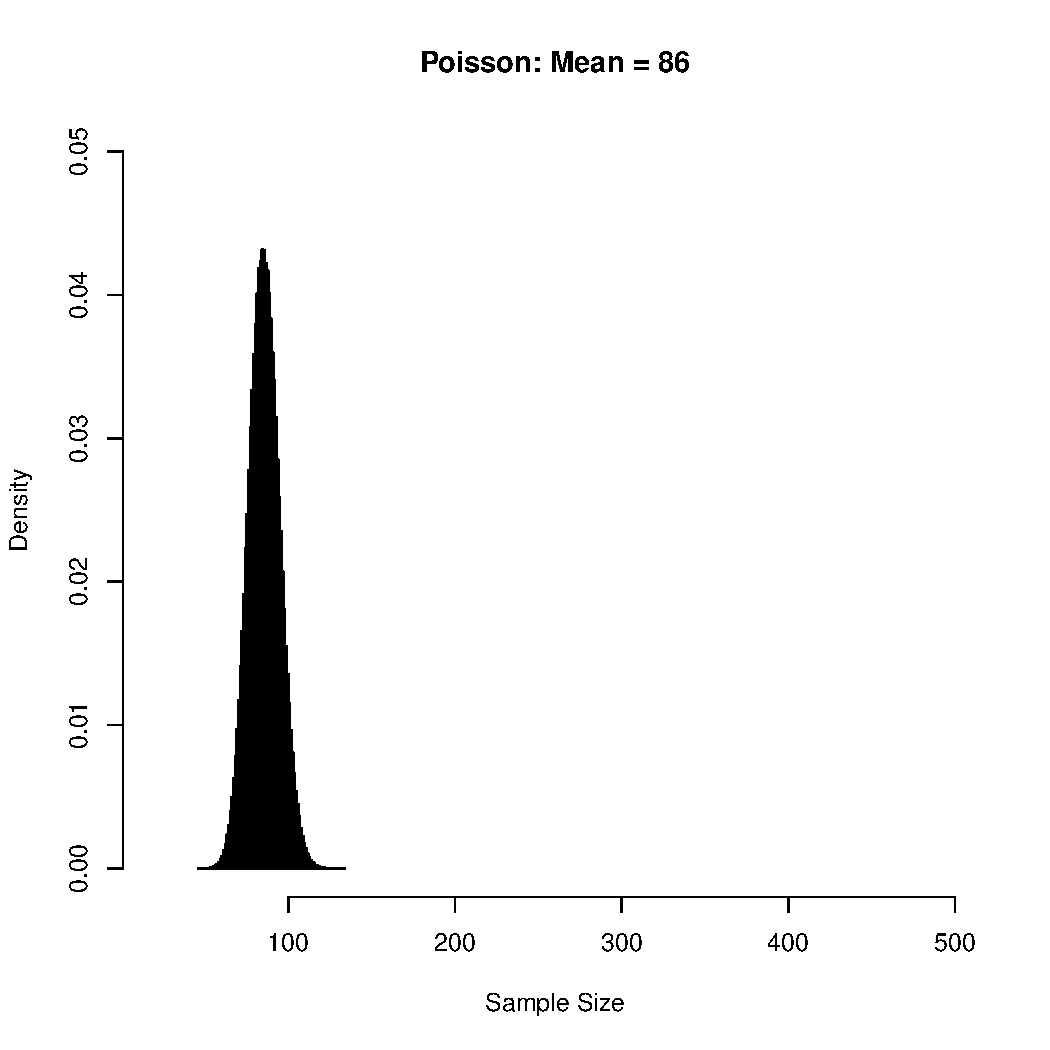
\includegraphics[width=3in]{pictures/Poisson} \\
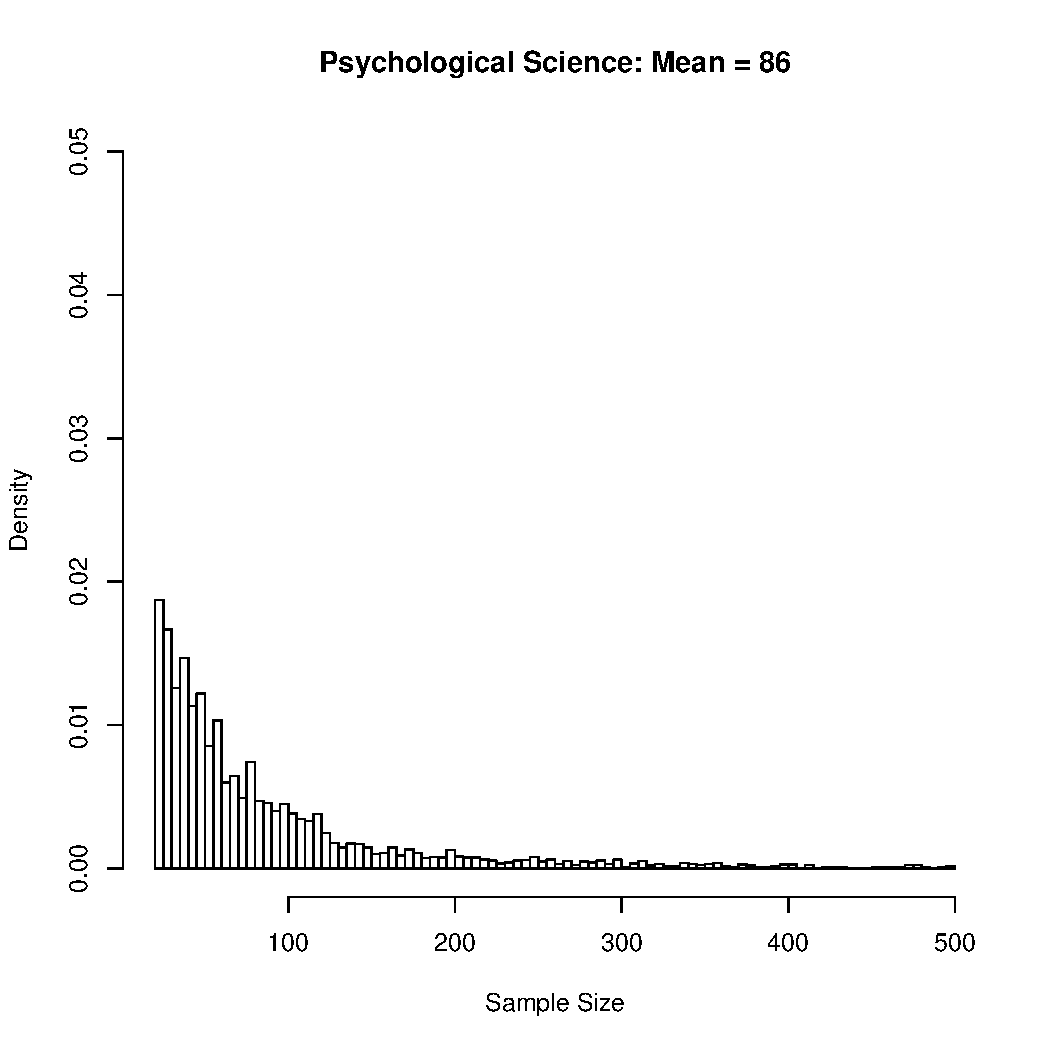
\includegraphics[width=3in]{pictures/PsychScience}
\end{tabular}
\end{center}\label{PoissonPsychScience} % Label after figure or numbering is wrong
\end{figure}

The \emph{Psychological Science} data consist of 7,000 pairs of numerator and denominator degrees of freedom. Actual sample sizes were not collected in this preliminary attempt at data mining, so sample size was approximated by $n = df_1+df_2+1$. Numerator degrees of freedom were limited to ten or fewer, and the data were edited so that sample size ranged from 20 to 500, with a mean of 86. 

\paragraph{Tests}

In the simulations under full heterogeneity, eighty percent of the tests were $F$-tests, and twenty percent were chi-squared. For the $F$-tests, $(df_1,df_2)$ pairs were randomly sampled with replacement from the \emph{Psychological Science} data. The degrees of freedom for the chi-squared tests were randomly sampled with replacement from the $df_1$ values. Sample sizes for the chi-squared tests were selected with replacement, independently of degrees of freedom. 

\paragraph{Effect size} 
In this set of simulations, effect size has a mixed continuous-discrete distribution. With probability 0.10, effect size equals zero, so that the null hypothesis is exactly true 10\% of the time. With probability 0.05, effect size has a standard exponential distribution shifted by one; in this case the minimum effect size is over twice
\citeauthor{Cohen1988}'s (\citeyear[][p.~287]{Cohen1988})``high" value for the $F$-test, representing manipulation checks and other ``findings" that are too good to be true. The other 0.85 probability is devoted to a beta distribution, with parameters chosen to make population mean power after selection either 0.25, 0.50 or 0.75. The same effect size distribution was used for chi-squared and $F$-tests even though the substantive meanings and power corresponding to a given effect size and sample size are different. No special attempt was made to hold the standard deviation of effect size constant, but all values were above the earlier ``high" value of 0.30. Sample size and effect size are independent after selection, so that before selection they are non-independent. This is a minor point, since we saw in the preceding section that correlation between sample size and effect size appears to make little difference.

Figure~\ref{EffectSizePower} shows the distribution of effect size after selection and and the resulting distribution of power after selection. The distribution of power includes the power of both chi-squared tests and $F$-tests. It is evident that the effect of heterogeneity in sample size and effect size is increased heterogeneity in power. Since power is bounded by 0.05 and one, its distribution is forced to the extremes.

\begin{figure} % [H] 
\caption{Distributions of effect size and power after selection, under full heterogeneity}
\begin{center}
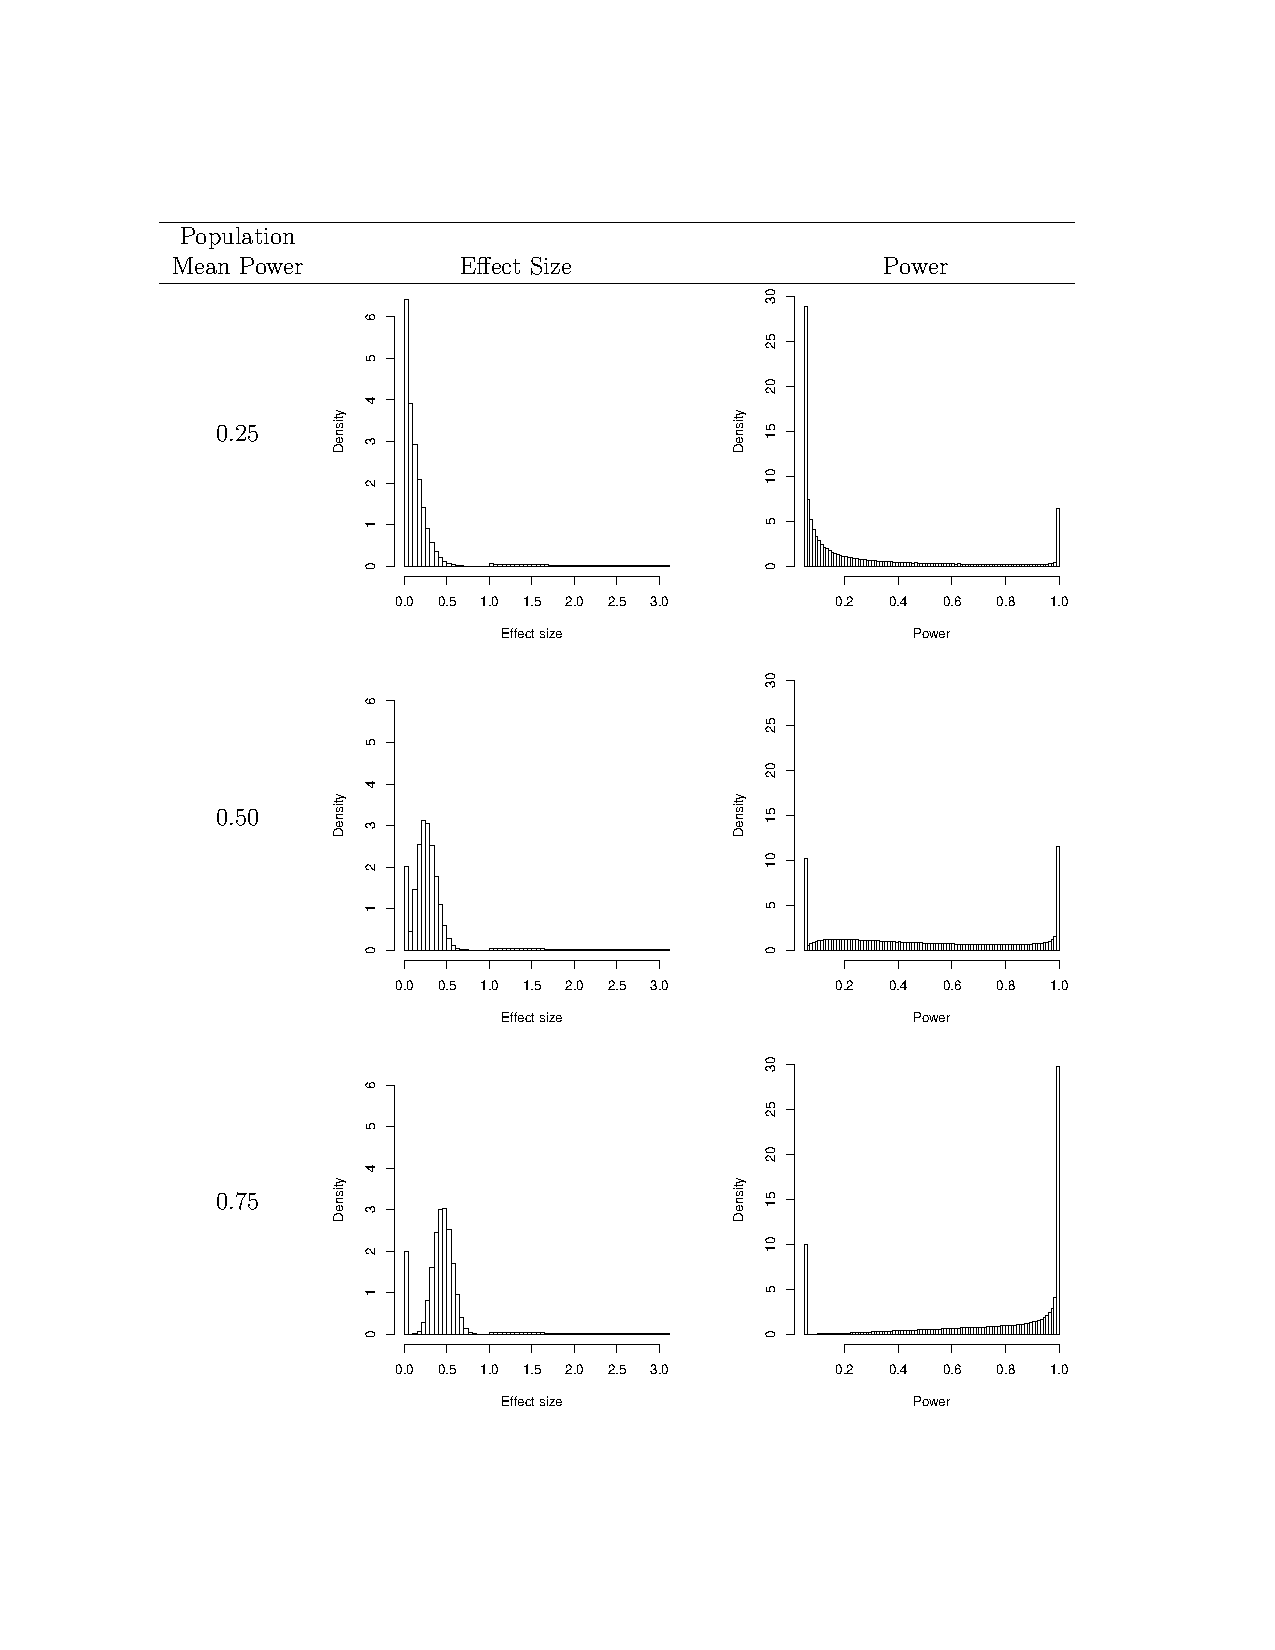
\includegraphics[width=3.4in]{pictures/ESpow}
\end{center} \label{EffectSizePower} % Label after figure or numbering is wrong
\end{figure}

% I cut and cropped the figure above from another document. Here is the original code.
% \begin{tabular}{ccc}
% \hline 
% Population && \\
% Mean Power &   Effect Size     &        Power       \\ \hline
% \raisebox{1.45in}{0.25} % R graphics are square, so 2x2 in this case -- raise 1
%      & 
\includegraphics[width=2.5in]{Pictures/FullES25}
%     & 
\includegraphics[width=2.5in]{Pictures/FullPOW25} \\
% \raisebox{1.45in}{0.50}
%      & 
\includegraphics[width=2.5in]{Pictures/FullES50}
%      & 
\includegraphics[width=2.5in]{Pictures/FullPOW50} \\
% \raisebox{1.45in}{0.75}
%      & 
\includegraphics[width=2.5in]{Pictures/FullES75}
%      & 
\includegraphics[width=2.5in]{Pictures/FullPOW75} \\
% \end{tabular}


\paragraph{Average performance} The p-curve~2.1, p-uniform, maximum likelihood and z-curve methods were used to estimate the means of the power distributions depicted in Figure~\ref{EffectSizePower}. Maximum likelihood continued to assume a gamma distribution for effect size, and independence of sample size and effect size before selection. For maximum likelihood, three sets of random starting values for the gamma parameters were employed. Table~\ref{fullmean} shows means of the estimates over 10,000 simulated sets of test statistics in each condition. The p-uniform method yields estimates that are much too high. P-curve~2.1 also over-estimates mean power, though to a much lesser degree than p-uniform. Over-estimation by p-curve~2.1 is most pronounced when true population mean power is high. Maximum likelihood and z-curve also yield mildly biased estimates, though not in a consistent direction across conditions. Overall, we judge the average estimates of maximum likelihood to be acceptable, and the average estimates of p-curve~2.1 to be acceptable when population mean power is low to medium. However, accuracy is more important than low estimation bias.

\begin{table}[h]
\caption{Average estimated population mean power under full heterogeneity}
{\small
\begin{center}
\begin{tabular}{lrrrrr c lrrrrr}  \hline
      & \multicolumn{5}{c}{$k=$ Number of Tests}  \\ 
      &  100  &  250   &  500   & 1000   & 2000  \\ \hline
\multicolumn{6}{l}{\textbf{Population Mean Power = 0.25}} \\ \hline
P-curve~2.1   & 0.280  & 0.280  & 0.283  & 0.288  & 0.292  \\
P-uniform & 0.691  & 0.776  & 0.823  & 0.856  & 0.877  \\
MaxLike   & 0.267  & 0.267  & 0.268  & 0.269  & 0.269   \\
Z-curve   & 0.251  & 0.240  & 0.234  & 0.232  & 0.230  \\ \hline
\multicolumn{6}{l}{\textbf{Population Mean Power = 0.50}} \\ \hline
P-curve~2.1   & 0.561  & 0.571  & 0.577  & 0.581  & 0.585 \\
P-uniform & 0.807  & 0.861  & 0.891  & 0.911  & 0.923 \\
MaxLike   & 0.473  & 0.468  & 0.465  & 0.463  & 0.462 \\
Z-curve   & 0.517  & 0.505  & 0.497  & 0.491  & 0.487 \\ \hline
\multicolumn{6}{l}{\textbf{Population Mean Power = 0.75}} \\ \hline
P-curve 2.1   & 0.828  & 0.836  & 0.840  & 0.842  & 0.844 \\
Puniform & 0.921  & 0.945  & 0.956  & 0.964  & 0.968 \\
MaxLike  & 0.740  & 0.736  & 0.734  & 0.731  & 0.730 \\
Zcurve   & 0.764  & 0.756  & 0.750  & 0.745  & 0.740 \\ \hline
\end{tabular}
\end{center}
} % End size
\label{fullmean}  % Label must come after the table or numbering is wrong. 
\end{table}

\paragraph{Absolute error of estimation} Table~\ref{fullabserr} shows mean absolute differences between the estimates and mean power, multiplied by 100. The p-uniform estimates are unacceptable, and p-curve~2.1 is clearly less accurate than maximum likelihood or z-curve. 
\begin{table} %[h]
\caption{Mean absolute error of estimation under full heterogeneity, in percentage points}
{\small
\begin{center}
\begin{tabular}{lrrrrr}  \hline
      & \multicolumn{5}{c}{Number of Tests} \\
           &  100  &  250   &  500   & 1000   & 2000 \\ \hline
      \multicolumn{6}{l}{\textbf{Population Mean Power = 0.25}} \\ \hline
P-curve~2.1    & 6.27  &  4.68  &  4.05  &  4.00  &  4.25 \\
P-uniform  & 44.14 & 52.57  & 57.35  & 60.56  & 62.67 \\
MaxLike    & 3.87  &  2.66  &  2.23  &  2.03  &  1.99 \\
Z-curve    & 5.13  &  3.53  &  2.95  &  2.60  &  2.43 \\ \hline
\multicolumn{6}{l}{\textbf{Population Mean Power = 0.50}} \\ \hline
P-curve~2.1    & 7.39  &  7.21  &  7.67  &  8.10  &  8.50 \\
P-uniform  & 30.67 & 36.14  & 39.13  & 41.06  & 42.30 \\
MaxLike    & 4.81  &  3.84  &  3.67  &  3.74  &  3.79 \\
Z-curve    & 5.93  &  3.78  &  2.81  &  2.23  &  1.98 \\ \hline
\multicolumn{6}{l}{\textbf{Population Mean Power = 0.75}} \\ \hline
P-curve~2.1    & 7.88  &  8.62  &  8.99  &  9.24  &  9.41 \\
P-uniform  & 17.11 & 19.48  & 20.61  & 21.36  & 21.84 \\
MaxLike    & 3.67  &  2.61  &  2.16  &  2.03  &  2.07 \\
Z-curve    & 3.64  &  2.45  &  1.81  &  1.48  &  1.38 \\ \hline
\end{tabular}
\end{center}
} % End size
\label{fullabserr}  % Label must come after the table or numbering is wrong. 
\end{table}
Table~\ref{fullabserr} suggests that maximum likelihood may have an advantage over z-curve when population mean power is low, while z-curve prevails when population mean power is medium to high. 

Within each of the 15 combinations of power and number of tests, there are six potential pairwise comparisons of mean accuracy. These comparisons were carried out using large-sample two-sided matched Z-tests with a Bonferroni correction at the joint 0.001 level. As would be anticipated from Table~\ref{fullabserr}, p-uniform was significantly less accurate than the other methods in all comparisons, and p-curve~2.1 was significantly less accurate than maximum likelihood and z-curve in all comparisons.
Table \ref{fullcontest} counts significant wins and losses; z-curve prevails over maximum likelihood by a score of seven to six. Five of maximum likelihood's six wins occur when the true population mean power is 0.25. In this setting, the z-curve estimate appears to settle down to 0.23 rather than 0.25 as the number of tests $k$ on which the estimate is based increases. This is not a serious error in practice. 

Note that while the distributional assumptions of maximum likelihood are violated in this simulation, it still performs approximately as well as z-curve. A glance at the upper left panel of Figure~\ref{EffectSizePower} suggests why. Even though the distribution of effect size is certainly not gamma, still the right-skewed and mostly decreasing distribution for low population mean power might be approximated fairly well be a gamma distribution.

\begin{table}[h]
\caption{Number of times row method is significantly more accurate than column method under full heterogeneity}
{\small
\begin{center}
\begin{tabular}{l ccccc }  \hline
          & P-curve~2.1  &  P-uniform & MaxLike & Z-curve &   Total  \\ \hline
P-curve~2.1   &    0     &      15    &    0    &   0     &     15   \\
P-uniform &    0     &       0    &    0    &   0     &      0   \\
MaxLike   &   15     &      15    &    0    &   6     &     36   \\
Z-curve   &   15     &      15    &    7    &   0     &     37   \\ \hline
\end{tabular}
\end{center}
} % End size
\label{fullcontest}  % Label must come after the table or numbering is wrong. 
\end{table}

\subsection{A conservative bootstrap confidence interval for z-curve}
Estimates should always be accompanied by confidence intervals, to give an idea of their precision. For z-curve, the most natural choice is a bootstrap confidence interval. The bootstrap
\parencite{Efron1979, EfronTibs1993} is based on re-sampling from the observed data with replacement, calculating a statistic on each re-sampled data set, and using the histogram of the resulting values as an approximation of the sampling distribution of the statistic. In this case the statistic is the z-curve estimate. Our choice is the percentile confidence interval method, which assumes that the sampling distribution of the estimate is symmetric, and centered on the quantity being estimated. Here, we re-sampled test statistics and computed z-curve estimates $B=500$ times. The 95 percent bootstrap confidence interval ranges from the 2.5 percentile to the 97.5 percentile of the estimates.  

Especially when samples are small, it is important to verify that a proposed 95\% confidence interval  contains the true value 95\% of the time. This is called the \emph{coverage} of the confidence interval. In a pilot study, we found that the coverage of the 95\% bootstrap confidence interval was sometimes less than 95\%. For example, notice in Table~\ref{fullmean} that the mean estimate for power = 0.25 and $k=2,000$ is 0.23 rather than 0.25. The sampling distribution of the z-curve estimate is nicely symmetric as required by the bootstrap method, but it is centered on 0.23 and not 0.25. The resulting coverage of the confidence interval is roughly 84\% when it should be 95. With increasing volume of data, the width of the confidence interval would shrink and the coverage would decrease to zero.

Reviewing the average z-curve estimates from all the simulations, we determined that the the bias of the z-curve estimate is seldom more than two percentage points, and never more than two percentage points for larger samples. Thus an easy fix of the confidence interval is to decrease the lower limit by 0.02 and increase the upper limit by 0.02. This yields our \emph{conservative bootstrap confidence interval}.

We tested the conservative bootstrap confidence interval in the setting of full heterogeneity, with 10,000 simulated datasets at each combination of three values of true population mean power (again, the distributions in Figure~\ref{EffectSizePower}), and seven values of the number of test statistics, ranging from $k=25$ to $k=2,000$. 

Table~\ref{coverage} gives the coverage values. Even for $k=25$ its performance is respectable. The table shows that the conservative bootstrap confidence interval is indeed conservative under most circumstances. When the estimates are based on larger numbers of test statistics, it behaves more like a 99 percent confidence interval. For estimates based on fewer than 25 test statistics, it might be helpful to increase the correction factor from 0.02 to 0.025. 

\begin{table} [H]
\caption{Coverage of the 95\% conservative bootstrap confidence interval}
{\scriptsize
\begin{center}
\begin{tabular}{c ccccccc }  \hline
Population & \multicolumn{7}{c}{Number of Tests} \\
Mean Power  &  25   &  50   &  100   &  250   &  500  & 1000  & 2000 \\ \hline
    0.25    & 95.78  & 97.13 & 98.02  & 98.69  & 98.76 & 98.35 & 97.95 \\
    0.50    & 94.58  & 95.51 & 96.79  & 98.27  & 99.11 & 99.28 & 99.15 \\
    0.75    & 93.21  & 94.81 & 96.83  & 98.85  & 99.37 & 99.73 & 99.58 \\ \hline
\end{tabular}
\end{center}
} % End size
\label{coverage}  % Label must come after the table or numbering is wrong. 
\end{table}

Table~\ref{meanlimits} shows mean upper and lower confidence limits. The upper limit is the top number in each cell, and the lower limit is the bottom number. For example, when the true population mean power is 0.75 and the z-curve estimate is based on $k=100$ test statistics, the average confidence interval will range from 0.65 to 0.85. This may be sufficient precision for some purposes, but it is desirable to base estimates on a larger number of test statistics if possible.
\begin{table}[H]
\caption{Average Upper and Lower Confidence limits}
{\small
\begin{center}
\begin{tabular}{c ccccccc }  \hline
Population & \multicolumn{7}{c}{Number of Tests} \\
Mean Power  &  25   &  50   &  100  &  250  &  500  & 1000  & 2000 \\ \hline
    0.25    & 0.54  & 0.46  & 0.40  & 0.35  & 0.32  & 0.30  &  0.29 \\
            & 0.06  & 0.09  & 0.11  & 0.14  & 0.16  & 0.17  & 0.17 \\
    0.50    & 0.76  & 0.71  & 0.67  & 0.62  & 0.58  & 0.56  & 0.55 \\
            & 0.26  & 0.32  & 0.36  & 0.39  & 0.41  & 0.42  & 0.43 \\
    0.75    & 0.89  & 0.87  & 0.85  & 0.83  & 0.81  & 0.80  & 0.79 \\
            & 0.55  & 0.61  & 0.65  & 0.67  & 0.68  & 0.69  & 0.69 \\ \hline
\end{tabular}
\end{center}
} % End size
\label{meanlimits}  % Label must come after the table or numbering is wrong. 
\end{table}
Table~\ref{meanlimits} suggests that estimating population mean power is fundamentally a large-sample game. When it is applied to smaller collections of studies, it is particularly important to accompany the estimates with confidence intervals. 

\section{Discussion}  % The discussion in Version 6.4 was more elaborate and detailed, including OSC.

In this paper, we have compared four methods for estimating the mean statistical power of a heterogeneous population of significance tests, after selection for significance. We have discovered and formally proved a set of fundamental principles relating the distribution of power values before selection to their distribution after selection. These principles were used extensively in a set of large-scale simulation studies comparing the estimation methods. For example, Principle~\ref{meansquaredovermean} states that population mean power after selection equals the population mean of squared power before selection, divided by population mean power before selection. This principle allowed the bivariate distribution of sample size and effect size before selection to be adjusted so that population mean power after selection would have exactly some desired value. Finding the right values by trial and error would have been extremely tedious, and never completely successful.

We used simulation to compare four methods for estimating population mean power after selection for significance: p-curve~2.1, p-uniform, maximum likelihood and z-curve.  We found that z-curve was the most accurate method when there was substantial heterogeneity in effect size and the distribution of effect size was unknown. Z-curve is also the most convenient, requiring only a set of $p$-values as input. Estimates should be accompanied by confidence intervals. We have provided a conservative bootstrap confidence interval for z-curve and verify by simulation that has good coverage even for small samples.

In a meta-analysis of studies testing exactly the same hypothesis with very similar subject populations, it is reasonable to assume that effect size is a single fixed constant, while sample size of course may vary. This is the setting for which p-curve~2.1 and p-uniform were designed. Here, all the methods performed reasonably well in our simulations. The most accurate method was maximum likelihood, followed by p-uniform. The original p-uniform method of \textcite{vanAssenEtAl2014} includes a high-quality confidence interval that extends readily to estimates of mean power. In simulation studies not reported here, we found the coverage of the p-uniform confidence intervals to be superior to coverage of the maximum likelihood confidence intervals, particularly for small samples. For this reason, we recommend the p-uniform method when there is strong reason to believe that heterogeneity in effect size is absent.

Then we introduced heterogeneity in effect size. In this situation, maximum likelihood estimates are based on a parametric model for the distribution of effect size, and also for the relationship between sample size and effect size. We carried out another large-scale simulation experiment in which effect size was gamma distributed and independent of sample size before selection. Maximum likelihood made full use of these features. When heterogeneity in effect size was moderate to high, maximum likelihood was by far the most accurate method in spite of numerical difficulties. The next most accurate was z-curve, which performed acceptably but not as well as maximum likelihood. The effect of high heterogeneity on p-uniform was particularly severe, leading to very high estimated mean power almost regardless of the true value. This confirms the view of the p-uniform team \parencite{vanAertEtAl2016}, who warn against using either p-curve~2.1 or p-uniform to estimate effect size when effect size is heterogeneous.

In practice, the probability distribution of effect size will never be known, and effect size may well be related to sample size. To test the robustness of maximum likelihood, we conducted a study in which effect size was beta distributed (limited to values between zero and one, in contrast to the assumed right-skewed gamma distribution), and the population correlation between sample size ranged from zero to -0.8. Maximum likelihood continued to assume a gamma distribution for effect size and zero correlation between sample size and effect size before selection. Here, z-curve was clearly more accurate than maximum likelihood, which in turn still out-performed p-curve~2.1 and p-uniform. The study provided strong evidence that maximum likelihood estimation of power is sensitive to violation of distributional assumptions, while correlation between sample size and effect size had little effect. In another simulation where effect size was right skewed but not gamma distributed, z-curve and maximum likelihood performed about equally well. We conclude that since the distribution of effect size is always unknown and moderate heterogeneity in effect size cannot be ruled out, the preferred method of estimating population mean power from published results is z-curve. 

Some important statistical features of z-curve require further investigation. One is the question of independence. In all our simulations, the input $p$-values were independent. While z-curve does not formally assume independent inputs, the bootstrap confidence interval definitely does. Further simulations could provide reassurance (or raise a warning flag) about the performance of the method when clusters of $p$-values come from tests conducted on the same data set. 

Another unresolved issue is how well the method z-curve method performs for tests that do not have one of the common non-central distributions under the alternative hypothesis. The most important case is in classical repeated measures ANOVA, where many test statistics have central $F$ distributions when the null hypothesis is true, but multiples of a central $F$ when the null hypothesis is false. Z-curve requires only $p$-values as input and can be computed immediately for such data, while special versions of the other methods would have to be developed. Conceptually, z-curve depends on estimating the approximate distribution of a latent non-centrality parameter. The question is how well it performs when there is no non-centrality parameter. Preliminary results are encouraging, but a full simulation study is needed. 

Neither the estimation methods we consider nor our simulations make any allowance for the kind of exploratory statistical analysis that capitalizes on chance, and makes statistical significance a near certainty. The terms ``vibration effects" \parencite{Ioannidis2008}, ``False-positive psychology" \parencite{SimmonsEtAl2011}, ``p-hacking" \parencite{SimonsohnEtAl2014a} and ``Questionable Research Practices" \parencite{uli2012} have been used. Here, we will call it p-hacking. We have no doubt that the practice of p-hacking is widespread and we suspect that it reduces the average true power of published studies. 

The question is how it influences \emph{estimates} of power. Simonsohn et al.~(2014b) report simulations that suggest optimism about the effect of p-hacking upon p-curve estimates of effect size. There is a need for larger-scale simulations that focus on the estimation of mean power and allow for heterogeneity in both sample size and effect size. Also, p-hacking can take a variety of different forms, and different p-hacking strategies may have different effects on the distribution of significant $p$-values. For example, stepwise regression results in lower average $p$-values than an optional stopping rule in which ``exploration" stops once $p < 0.05$. Variation in p-hacking strategy needs to be explored. Only when we understand the effects of p-hacking on estimated power, particularly when true power is greater than 0.05, will we be able to confirm the potential accuracy of z-curve for real data.


\printbibliography

\section{Appendix}

\subsection{Proofs of the Principles, with an example}

This section of the appendix contains formal proofs of the Principles given in \emph{Two populations of power}. The principles are also illustrated with a numerical example. Consider a population of $F$-tests with 3 and 26 degrees of freedom, and varying true power values. Variation in power comes from variation in the non-centrality parameter, which is sampled from a chi-squared distribution with degrees of freedom chosen so that population mean power is very close to 0.80. 

Denoting a randomly selected power value by $G$ and the non-centrality parameter by $\lambda$, population mean power is
\begin{displaymath}
    E(G) =  \int_0^\infty (1-\R{pf(}c,\R{ncp}=\lambda\R{)})  \, \R{dchisq(}\lambda\R{)} \, d\lambda
\end{displaymath}
To verify the numerical value of expected power for the example,
% Being careful to make the R material fit into a single column on the typeset page ... 
{\footnotesize
\begin{verbatim}
> alpha = 0.05; criticalvalue = qf(1-alpha,3,26)
> fun = function(ncp,DF)
+   (1 - pf(criticalvalue,df1=3,df2=26,ncp))*dchisq(ncp,DF)
> integrate(fun,0,Inf,DF=14.36826)
0.8000001 with absolute error < 5.9e-06
\end{verbatim}
} % End size
\noindent
The strange fractional degrees of freedom were located using the R function \texttt{uniroot}, minimizing the absolute difference between the output of \texttt{integrate} and the value 0.8 numerically over the degrees of freedom value. The minimum occurred at 14.36826.

\textbf{Principle \ref{doubleex}} states that \emph{Population mean true power equals the overall probability of a significant result.}
\paragraph{Proof} 
Suppose that the distribution of true power is discrete. Again denoting a randomly chosen power value by $G$, the probability of rejecting the null hypothesis is 
\begin{eqnarray} \label{ExpectedPow}
    Pr\{T>c\} & = & \sum_g Pr\{T>c|G=g\} Pr\{G=g\}  \nonumber \\
    & = & \sum_g g \, Pr\{G=g\}  \nonumber \\
    & = & E(G),
\end{eqnarray}
which is population mean power. If the distribution of power is continuous with probability density function $f_{_G}(g)$, the calculation is 
\begin{eqnarray*}
    Pr\{T>c\} & = & \int_0^1 Pr\{T>c|G=g\} f_{_G}(g) \, dg \\
    & = & \int_0^1 g \, f_{_G}(g) \, dg \\
    & = & E(G) ~~~\blacksquare
\end{eqnarray*}
Continuing with the numerical example, we first sample one million non-centrality parameter values from the chi-squared distribution that yields an expected power of 80\%. These values are in the vector \texttt{NCP}. We then calculate the corresponding power values, placing them in the vector \texttt{Power}. Next, we generate one million random $F$ statistics from non-central $F$ distributions, using the non-centrality parameter values in \texttt{NCP}. In the R output below, observe that mean power is very close to the proportion of $F$ statistics exceeding the critical value. This illustrates Principle~\ref{doubleex} for the distribution of power before selection. Needless to say, Principle~\ref{doubleex} applies both before and after selection. 

{\footnotesize
\begin{verbatim}
> popsize = 1000000; set.seed(9999)
> NCP = rchisq(popsize,df=14.36826)
> Power = 1 - pf(criticalvalue,df1=3,df2=26,NCP)
> mean(Power)
[1] 0.8002137
> Fstat = rf(popsize,df1=3,df2=26,NCP)
> sigF = subset(Fstat,Fstat>criticalvalue)
> length(sigF)/popsize # Proportion significant
[1] 0.800177
\end{verbatim}
} % End size

To show how Principle~\ref{doubleex} applies to the distribution of power after selection, the sub-population of power values corresponding to significant results are stored in \texttt{SigPower}. The tests that were significant are repeated (with the same non-centrality parameters), and the test statistics placed in \texttt{Fstat2}. The proportion of test statistics in \texttt{Fstat2} that are significant is very close to the mean of \texttt{SigPower}. This gives empirical support to the statement that population mean power after selection for significance equals the probability of obtaining a significant result again.

{\footnotesize
\begin{verbatim}
> SigPower = subset(Power,Fstat>criticalvalue)
> mean(SigPower) # Mean power after selection
[1] 0.8274357
> # Replicate the tests that were significant.
> sigNCP = subset(NCP,Fstat>criticalvalue)
> Fstat2 = rf(length(sigF),df1=3,df2=26,ncp=sigNCP)
> # Proportion of replications significant
> length(subset(Fstat2,Fstat2>criticalvalue)) / 
+                                   length(sigF)
[1] 0.827172
\end{verbatim}
} % End size

\textbf{Principle \ref{pdf}} states that \emph{the effect of selection for significance is to multiply the probability of each power value by a quantity equal to the power value itself, divided by population mean power before selection. If the distribution of power is continuous, this statement applies to the value of the probability density function.}
\paragraph{Proof} Suppose the distribution of power is discrete. Using Bayes' Theorem, 
\begin{equation} \label{CondProb}
    Pr\{G=g|T>c\} = \frac{Pr\{T>c|G=g\} Pr\{G=g\}}{Pr\{T>c\}} = \frac{g \, Pr\{G=g\}}{E(G)}.
\end{equation}
If the distribution of power is continuous with density $f_{_G}(g)$,
\begin{eqnarray*}
    Pr\{G \leq g|T>c\} & = &  \frac{Pr\{G \leq g, T>c\}}{Pr\{T>c\}}  \\
    & = &  \frac{\int_0^g Pr\{T>c|G=x\} f_{_G}(x) \, dx }{E(G)}  \\
    & = &  \frac{\int_0^g x \, f_{_G}(x) \, dx }{E(G)}. 
\end{eqnarray*}
By the Fundamental Theorem of Calculus, the conditional density of power given significance is
\begin{equation} \label{CondDens}
    \frac{d}{dg}Pr\{G \leq g|T>c\} = \frac{g \, f_{_G}(g)}{E(G)}.~~~\blacksquare
\end{equation}

For the numerical example we are pursuing by simulation, the density function of power before selection is a technical challenge and we will not attempt it. As a substitute, suppose that power before selection follows a beta distribution, a very flexible family on the interval from zero to one \parencite{JohnsonEtAl1995}. If power before selection (denoted by $G$) has a beta distribution with parameters $\alpha$ and $\beta$, Principle~\ref{pdf} says that the density of power after selection (a function of the power value $g$) is
\begin{eqnarray*}
    f(g|T>c)
    &=& \frac{\Gamma(\alpha+\beta)}{\Gamma(\alpha)\Gamma(\beta)} g^{\alpha-1}(1-g)^{\beta-1} 
        \left( \frac{g}{E(G)} \right) \\
    &=& \left( \frac{1}{\alpha/(\alpha+\beta)} \right)
    \frac{\Gamma(\alpha+\beta)}{\Gamma(\alpha)\Gamma(\beta)} g^{\alpha}(1-g)^{\beta-1}  \\
    &=& \frac{(\alpha+\beta) \, \Gamma(\alpha+\beta)} {\alpha \, \Gamma(\alpha) \, \Gamma(\beta)} 
        g^{\alpha+1-1}(1-g)^{\beta-1} \\
    &=& \frac{\Gamma(\alpha+1+\beta)}{\Gamma(\alpha+1) \, \Gamma(\beta)} g^{\alpha+1-1}(1-g)^{\beta-1},
\end{eqnarray*}
which remarkably is again a beta density, this time with parameters $\alpha+1$ and $\beta$. Figure~\ref{pdfmult3} shows how a beta with $\alpha=2$ and $\beta=4$ is transformed into a beta with $\alpha=3$ and $\beta=4$.
\begin{figure}[h] 
\caption{Beta density of power before and after selection}
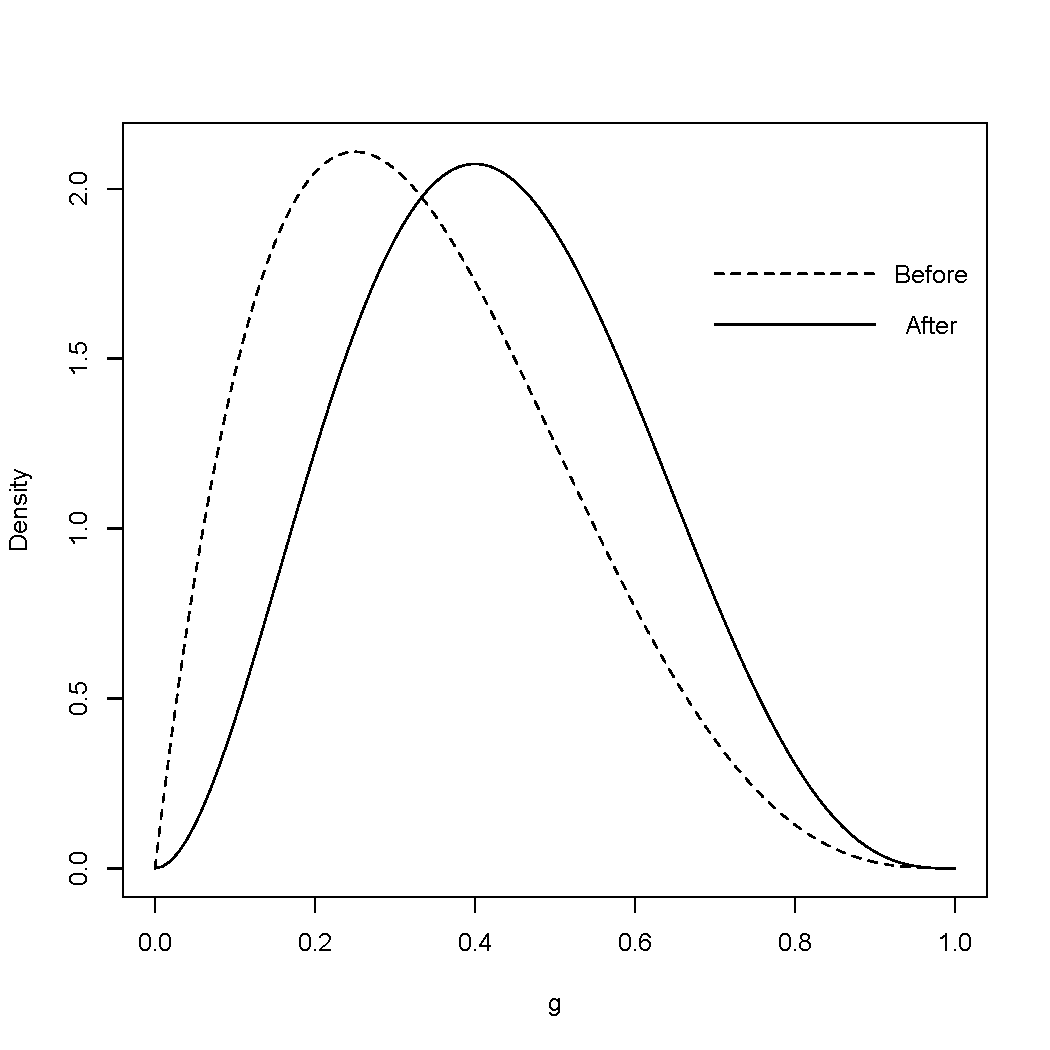
\includegraphics[width=3in]{pictures/betadens} 
\label{pdfmult3} % Label after figure or numbering is wrong
\end{figure}

\textbf{Principle \ref{meansquaredovermean}} states that \emph{Population mean power after selection for significance equals the population mean of squared power before selection, divided by the population mean of power before selection.}.

\paragraph{Proof} Suppose that the distribution of power is discrete. Then using~(\ref{CondProb}), 
\begin{equation} \label{ExpectedPowGivenSig1}
    E(G|T>c) = \sum_g \, g \, \frac{g \, Pr\{G=g\}}{E(G)} = \frac{E(G^2)}{E(G)}.
\end{equation}
If the distribution of power is continuous,  (\ref{CondDens}) is used to obtain
\begin{equation} \label{ExpectedPowGivenSig2}
    E(G|T>c) = \int_0^1 \, g \, \frac{g \, f_{_G}(g)}{E(G)} \, dg = \frac{E(G^2)}{E(G)}.
    ~~~\blacksquare
\end{equation} 
In the example, \texttt{SigPower} contains the sub-population of power values corresponding to significant results. Observe the verification of Formula~\ref{ExpectedPowGivenSig2}.

{\footnotesize
\begin{verbatim}
> # Repeating ...
> SigPower = subset(Power,Fstat>criticalvalue)
> mean(SigPower)
[1] 0.8274357
> mean(Power^2)/mean(Power)
[1] 0.8275373
\end{verbatim}
} % End size

\textbf{Principle \ref{recip}} states that \emph{population mean power before selection equals one divided by the population mean of the reciprocal of power after selection.}.

\paragraph{Proof} Using Formula~\ref{CondProb}, 
\begin{eqnarray*}
      E\left(\left.\frac{1}{G}\right|T>c \right) 
      &=& \sum_g \left(\frac{1}{g}\right) \frac{g \, Pr\{G=g\}}{E(G)} \nonumber \\
      &=& \frac{1}{E(G)}\sum_g Pr\{G=g\} = \frac{1}{E(G)} \cdot 1 \nonumber \\
      &=& \frac{1}{E(G)},
\end{eqnarray*}
so that
\begin{equation*} 
    E(G) = 1\left/ E\left(\left.\frac{1}{G}\right|T>c \right) \right. .
\end{equation*}
A similar calculation applies in the continuous case. $\blacksquare$

\vspace{3mm}

\noindent
To illustrate Principle~\ref{recip}, recall that the example was constructed so that mean power before selection was equal to 0.80.
{\footnotesize
\begin{verbatim}
> 1/mean(1/SigPower)
[1] 0.8000502
\end{verbatim}
} % End size

In the example, population mean power is 0.80, while population mean power given significance is roughly 0.83. It is reasonable that selecting significant tests would also tend to select higher power values on average, and in fact this intuition is correct. Since
\begin{eqnarray*}
      Var(G) &=& E(G^2) - \left(E(G)\right)^2 \geq 0, \mbox{ we have} \\
      E(G^2) & \geq & \left(E(G)\right)^2, \mbox{ and hence}\\
      \frac{E(G^2)}{E(G)} &\geq& E(G).
\end{eqnarray*}
Principle~\ref{meansquaredovermean} says $\frac{E(G^2)}{E(G)} = E(G|T>c)$, so that $E(G|T>c) \geq E(G)$. That is, population mean power given significance is greater than the mean power of the entire population, except in the homogeneous case where $Var(G)=0$. The exact amount of increase has a compact and somewhat surprising form.

\textbf{Principle \ref{increase}} states that \emph{the increase in population mean power due to selection for significance equals the population variance of power before selection divided by the population mean of power before selection.}.

\paragraph{Proof} 
\begin{eqnarray*} \label{Increase}
  E(G|T>c) - E(G) &=& \frac{E(G^2)}{E(G)} - E(G) \\
                  &=& \frac{E(G^2)}{E(G)} - \frac{\left(E(G)\right)^2}{E(G)} \\
                  &=& \frac{Var(G)}{E(G)}.  ~~~\blacksquare
\end{eqnarray*}
Illustrating Principle~\ref{increase} for the ongoing example,
{\footnotesize
\begin{verbatim}
> mean(SigPower) - mean(Power)
[1] 0.02722205
> var(Power)/mean(Power)
[1] 0.02732371
\end{verbatim}
} % End size

\textbf{Principle \ref{jointNes}} says that \emph{the effect of selection for significance is to multiply the joint distribution of sample size and effect size by power for that sample size and effect size, divided by population mean power before selection.}

\paragraph{Proof} Note that power for a given sample size and effect size is $P\{T>c|X=\R{es},N=n\}$. Suppose effect size is discrete. Then $P\{X=\R{es},N=n|T>c\}$ is 
\begin{eqnarray*}
    &   & \frac{P\{X=\R{es},N=n,T>c\}}{P\{T>c\}} \\
    & = & \frac{ P\{T>c|X=\R{es},N=n\}P\{X=\R{es},N=n\} }{E(G)} \\
    & = & \left( \frac{ P\{T>c|X=\R{es},N=n\} }{E(G)} \right) P\{X=\R{es},N=n\} \, ,
\end{eqnarray*}
where  $E(G)$ is expected power before selection, equal to $P\{T>c\}$ by Principle~\ref{doubleex}.

Suppose that effect size is continuous with density $g(\R{es})$. The joint distribution of sample size and effect size before selection is determined by $P\{N=n|X=\R{es}\}g(\R{es})$. The joint distribution after selection is determined by \\ $P\{N=n|X=\R{es},T>c\}\,g(\R{es}|T>c)$
{\small
\begin{eqnarray*}
    & = & 
   \frac{P\{T>c|X=\R{es},N=n\}P\{N=n|X=\R{es}\}g(\R{es})}
        {g(\R{es}|T>c)P\{T>c\}}  g(\R{es}|T>c) \\
    & = & 
    \left( \frac{ P\{T>c|X=\R{es},N=n\} }{E(G)} \right)
    P\{N=n|X=\R{es}\}g(\R{es})  \, .
\end{eqnarray*}
} % End size

\noindent
It is also possible to write the joint distribution of sample size and effect size as the conditional density of effect size given sample size, times the discrete probability of sample size. That is, the joint distribution before selection is determined by $g(\R{es}|N=n)P\{N=n\}$, and the joint distribution after selection is determined by $g(\R{es}|N=n,T>c)P\{N=n|T>c\}$
{\small
\begin{eqnarray} \label{joynt}
    & = & 
    \frac{d}{d\R{es}} P\{X\leq\R{es}|N=n,T>c\}P\{N=n|T>c\} \nonumber \\
    & = & \frac{d}{d\R{es}}
    \frac{ P\{X\leq\R{es},N=n,T>c\} }{ P\{N=n,T>c\} } 
    \frac{P\{N=n,T>c\}}{P\{T>c\}} \nonumber \\
    & = & \frac{1}{E(G)} \frac{d}{d\R{es}}
    \int_0^{\scriptsize \R{es}} 
    P\{T>c|X=y,N=n\} g(y|N=n)P\{N=n\} \, dy \nonumber \\
    & = & 
    \frac{P\{T>c|X=\R{es},N=n\}g(\R{es}|N=n)P\{N=n\} }{E(G)} \nonumber \\
     & = &
     \left( \frac{ P\{T>c|X=\R{es},N=n\} }{E(G)} \right)
     g(\R{es}|N=n)P\{N=n\} ~~ \blacksquare
\end{eqnarray}
} % End size

Principle~\ref{jointNes} cannot be illustrated for the ongoing numerical example, because the example employs a distribution of the non-centrality parameter, rather than of sample size and effect size jointly. As a substitute, consider that an observed distribution of sample size after selection must imply a distribution of sample size in the unpublished studies before selection. If that distribution is too outlandish (for example, implying an enormous ``file drawer" of pilot studies with tiny sample sizes) we may be forced to another model of the research and publication process. Principle~\ref{jointNes} allows one to solve for $P\{N=n\}$, the unconditional probability distribution of sample size before selection, though an estimated or hypothesized distribution of effect size given sample size before selection is needed. When sample size and effect size are deemed independent before selection, this is not a serious obstacle.

%First, observe that $P\{N=n|T>c\}$ is the distribution of sample size after selection, which is easy to estimate from data. The quantity $P\{T>c|X=\R{es},N=n\}$ is just power as a function of sample size and effect size. %In the R-like notation introduced at the beginning of the paper, Expression~\ref{powereq} says $P\{T>c|X=\R{es},N=n\} = 1-\R{p(}c,f_1(n)\cdot f_2(\R{es})\R{)}$.
Expression~\ref{joynt} says that $g(\R{es}|N=n,T>c)P\{N=n|T>c\}$ is equal to
{\small
\begin{displaymath} 
    \left( \frac{ P\{T>c|X=\R{es},N=n\} }{E(G)} \right) g(\R{es}|N=n)P\{N=n\},
\end{displaymath}
} % End size
so that integrating both sides with respect to \texttt{es},
{\small
\begin{eqnarray*} 
    &&  \int g(\R{es}|N=n,T>c)P\{N=n|T>c\} \, d\R{es} \\
    &=& P\{N=n|T>c\} \int g(\R{es}|N=n,T>c) \, d\R{es} \\
    &=& P\{N=n|T>c\} ~ \cdot ~ 1 \\
    &=& \int \left( \frac{ P\{T>c|X=\R{es},N=n\} }{E(G)} \right) 
        g(\R{es}|N=n)P\{N=n\} \, d\R{es} \\
    &=& \left(\frac{P\{N=n\}}{E(G)} \right) 
        \int  P\{T>c|X=\R{es},N=n\} \, g(\R{es}|N=n) \, d\R{es}, \\
\end{eqnarray*}
} % End size
and we have
{\small
\begin{equation} \label{Pn}
    P\{N=n\} = E(G) \left(\frac{P\{N=n|T>c\}}
               {\int P\{T>c|X=\R{es},N=n\}\,g(\R{es}|N=n)\,d\R{es} }
                   \right)
\end{equation}
} % End size

The numerator of the fraction is the probability of observing a sample size of $n$ after selection for significance. The denominator is expected power given that sample size, and could be calculated with R's \texttt{integrate} function. By Principle~\ref{doubleex}, the quantity $E(G)$ is both population mean power before selection and $P\{T>c\}$, the probability of randomly choosing a significant result from the population of tests before selection. In Equation~\ref{Pn}, though, it is just a proportionality constant. In practice, one obtains $P\{N=n\}$ by calculating the fraction in parentheses for each $n$, and then dividing by the total to obtain numbers that add to one.

\subsection*{Maximum Likelihood}

Even though sample size is a random variable, the quantities $n_1, \ldots, n_k$ are treated as fixed constants. This is similar to the way that $x$ values in normal regression and logistic regression are treated as fixed constants in the development of the theory, even though clearly they are often random variables in practice. Making the estimation conditional on the observed values $n_1, \ldots, n_k$ allows it to be distribution free with respect to sample size, just as regression and logistic regression are distribution free with respect to $x$. This is preferable to adopting parametric assumptions about the joint distribution of sample size and effect size.


Suppose there is heterogeneity in both sample size and effect size, and that effect size is continuous. The likelihood function given significance is a product of conditional densities evaluated at the observed values of the test statistics.
%, and viewed as a function of the unknown parameters. 
Each term is the conditional density of the test statistic given both the sample size and the event that the test statistic exceeds its respective critical value.  % The unknown parameters are the parameters of the distribution of effect size.

The joint probability distribution of sample size and effect size before selection is determined by the marginal distribution of sample size $P\{N=n\}$ and the conditional density of effect size given sample size $g_\theta(\R{es}|n)$, where $\theta$ is a vector of unknown parameters. 
Denoting the random effect size by $X$, the conditional density of an observed test statistic $T$ given significance and a particular sample size $n$ is
{\small
\begin{eqnarray*}
    &&    \frac{d}{dt} P\{T\leq t| T >c, N=n \} \\
    & = & \frac{d}{dt} \, \frac{P\{T \leq t, T> c, N=n \}}
                                  {P\{T>c, N=n\}}  \\
    & = & \frac{d}{dt} \, \frac{P\{c< T \leq t| N=n \} P\{N=n\}}         
                               {P\{T>c| N=n\} P\{N=n\}} \\
    & = & \frac{d}{dt} \, \frac{P\{c< T \leq t| N=n \}}         
                               {P\{T>c| N=n\}} \\     % Could cut this step
    & = & \frac{d}{dt} \, 
          \frac{\int_0^\infty P\{c< T \leq t| N=n,X=\R{es}\} g_\theta(\R{es}|n) \, d\R{es}}
               {\int_0^\infty P\{T>c| N=n,X=\R{es}\}  g_\theta(\R{es}|n) \, d\R{es}} \\  
    & = & \frac{d}{dt} \, 
          \frac{\int_0^\infty \left[\R{p(}t\R{,}f_1(n)f_2(\R{es})\R{)} -
                \R{p(}c\R{,}f_1(n)f_2(\R{es})\R{)} \right] g_\theta(\R{es}|n) \, d\R{es} }
               {\int_0^\infty \left[1-\R{p(}c\R{,}f_1(n)f_2(\R{es})\R{)}\right] 
                g_\theta(\R{es}|n) \, d\R{es} } \\
    & = & \frac{\int_0^\infty \frac{d}{dt} \R{p(}t\R{,}f_1(n)f_2(\R{es})\R{)}
                g_\theta(\R{es}|n) \, d\R{es}} 
               {\int_0^\infty\left[1-\R{p(}c\R{,}f_1(n)f_2(\R{es})\R{)}\right]
                g_\theta(\R{es}|n) \, d\R{es}} \\
    & = & \frac{\int_0^\infty\R{d(}t\R{,}f_1(n)f_2(\R{es})\R{)} 
                g_\theta(\R{es}|n) \, d\R{es}} 
               {\int_0^\infty\left[1-\R{p(}c\R{,}f_1(n)f_2(\R{es})\R{)}\right]
                g_\theta(\R{es}|n) \, d\R{es}} ~,
\end{eqnarray*} 
} % End size to fit the equations in the 2-column format.
where moving the derivative through the integral sign is justified by dominated convergence. The likelihood function is a product of $k$ such terms. In the main paper, the simplifying assumption that sample size and effect size are independent before selection means that $g_\theta(\R{es}|n)$ is replaced by $g_\theta(\R{es})$, yielding Expression~(\ref{likehetero}). 

In the problem of estimating power under heterogeneity in effect size, the unknown parameter is the vector $\theta$ in the density of effect size. Let $\widehat{\theta}$ denote the maximum likelihood estimate of $\theta$. This yields a maximum likelihood estimate of the true power of each individual test in the sample, and then the estimates are averaged to obtain an \nopagebreak estimate of mean power. We now give details.

Consider randomly sampling a single test from the population of tests that were significant the first time they were carried out. Let $T_1$ denote the value of the test statistic the first time a hypothesis is tested, and let $T_2$ denote the value of the test statistic the second time that particular hypothesis is tested, under exact repetition of the experiment. Conditionally on fixed values of sample size $n$ and effect size \texttt{es}, $T_1$ and $T_2$ are independent. By Principle~\ref{doubleex}, population mean power after selection is
{\small
\begin{equation} \label{probsig2givensig1}
    P\{ T_2 > c | T_1 > c\} = \sum_n P\{T_2>c | T_1>c, N=n \} P\{N=n|T_1>c\}
\end{equation}
} % End size
This is the expression we seek to estimate. Applying Principle~\ref{meansquaredovermean} to the sub-population of tests based on a sample of size $n$,

{\small
\begin{eqnarray} \label{ratiogivenN}
    & &    P\{T_2>c | T_1>c, N=n  \} \nonumber \\
    & = & \frac{ E(G^2|N=n) }
                                         { E(G|N=n) }               \nonumber       \\
    & = & \frac{\int_0^\infty\left[1-\R{p(}c\R{,}f_1(n)f_2(\R{es})\R{)}\right]^2
      g_{\theta}(\R{es}|n) \, d\R{es}} 
     {\int_0^\infty\left[1-\R{p(}c\R{,}f_1(n)f_2(\R{es})\R{)}\right]
      g_{\theta}(\R{es}|n) \, d\R{es}} \, .
\end{eqnarray}
} % End size

Substituting (\ref{ratiogivenN}) into (\ref{probsig2givensig1}) yields
$ P\{ T_2 > c | T_1 > c\} =$
{\small
\begin{equation} \label{Probsig2givensig1}
    \sum_n 
    \frac{\int_0^\infty\left[1-\R{p(}c\R{,}f_1(n)f_2(\R{es})\R{)}\right]^2
      g_{\theta}(\R{es}|n) \, d\R{es}} 
     {\int_0^\infty\left[1-\R{p(}c\R{,}f_1(n)f_2(\R{es})\R{)}\right]
      g_{\theta}(\R{es}|n) \, d\R{es}} P\{N=n|T_1>c\} \, .
\end{equation}
} % End size
Expression \ref{Probsig2givensig1} has two unknown quantities, the parameter $\theta$ of the effect size distribution, and $P\{N=n|T_1>c\}$. For the former quantity, we use the maximum likelihood estimate, while the $P\{N=n|T_1>c\}$ values are estimated by the empirical relative frequencies of sample size, which is the non-parametric maximum likelihood estimate. The result is a maximum likelihood estimate of population power given significance:
\begin{equation*} % \label{}
    \frac{1}{k} \sum_{j=1}^k 
    \frac{\int_0^\infty\left[1-\R{p(}c_j\R{,}f_1(n_j)f_2(\R{es})\R{)}\right]^2
      g_{\widehat{\theta}}(\R{es}|n_j) \, d\R{es}} 
     {\int_0^\infty\left[1-\R{p(}c_j\R{,}f_1(n_j)f_2(\R{es})\R{)}\right]
      g_{\widehat{\theta}}(\R{es}|n_j) \, d\R{es}}  \, .
\end{equation*}
In the simulations, the density $g$ of effect size is assumed gamma, there is no dependence on $n$, and the parameter $\theta$ is the pair $(a,b)$ that parameterize the gamma distribution.

\subsection{Simulation}

\paragraph{Direct simulation from the distribution of the test statistic given significance}
To study the behaviour of an estimation method under selection for significance, it is natural to simulate test statistics from the distribution that applies before selection, and then discard the ones that are not significant. But if one can simulate from the joint distribution of sample size and effect size after selection, the wasteful discarding of non-significant test statstics can be avoided. The idea is to do the simulation in two stages. First, simulate pairs from the joint distribution of sample size and effect size after selection, and calculate a non-centrality parameter using Expression~(ncpmult). Then using that \texttt{ncp} value, simulate from the distribution of the test statistic given significance. We will now show how to do the second step.

It is well known that if $F(t)$ is a cumulative distribution function of a continuous random variable
and $U$ is uniformly distributed on the interval from zero to one, then the random variable $T=F^{-1}(U)$ has cumulative distribution function $F(t)$. In this case the cumulative distribution function from which we wish to simulate is $P\{T \leq t | T>c, X=\R{es}, N=n \} $
%{\small
\begin{eqnarray*}
    & = & \frac{ P\{T \leq t, T>c | X=\R{es}, N=n\} }{ P\{T>c | X=\R{es}, N=n\} } \\
    & = & \frac{ P\{c < T \leq t | X=\R{es}, N=n\} }{ P\{T>c | X=\R{es}, N=n\} } \\
    & = & \frac{ \R{p(}t\R{,ncp)}-\R{p(}c\R{,ncp)} } { 1-\R{p(}c\R{,ncp)} }
\end{eqnarray*}
%} % End size
for $t>c$, where as usual $\R{ncp} = f_1(n)f_2(\R{es})$. To obtain the inverse, set $u$ equal to the probability and solve for $t$, as follows. Denoting the power of the test by $\gamma = 1-\R{p(}c\R{,ncp)}$,
%{\small
\begin{eqnarray*}
    && u =  \frac{ \R{p(}t\R{,ncp)}-\R{p(}c\R{,ncp)} } { 1-\R{p(}c\R{,ncp)} }   \\
    & \Leftrightarrow & 
    u \left(1-\R{p(}c\R{,ncp)}\right) = \R{p(}t\R{,ncp)}-\R{p(}c\R{,ncp)}       \\ 
    & \Leftrightarrow &
    \R{p(}t\R{,ncp)} = u \left(1-\R{p(}c\R{,ncp)}\right) + \R{p(}c\R{,ncp)}     \\
    & \Leftrightarrow &
    \R{p(}t\R{,ncp)} = \gamma u+1-\gamma                                        \\
    & \Leftrightarrow &
    t = \R{q(}\gamma u+1-\gamma\R{,ncp)}.
\end{eqnarray*}
%} % End size
Accordingly, let $U$ be a Uniform (0,1) random variable. The significant test statistic is
%{\small
\begin{eqnarray*}
    T & = & \R{q(}\gamma U+1-\gamma\R{,ncp)} \\
      & = & \R{q(}1+\gamma (U-1)\R{,ncp)}      \\
      & = & \R{q(}1-\gamma (1-U)\R{,ncp)} \, .
\end{eqnarray*}
%} % End size
Since $1-U$ also has a Uniform (0,1) distribution, one may proceed as follows. For a given sample size and effect size, first calculate the non-centrality parameter $\R{ncp} = f_1(n)f_2(\R{es})$, and use that to compute the power value $\gamma = 1-\R{p(}c\R{,ncp)}$. Then calculate the significant test statistic 
\begin{equation} \label{sigstat}
    T = \R{q(}1-\gamma U\R{,ncp)} \, ,
\end{equation}
where $U$ is a pseudo-random variate from a Uniform (0,1) distribution. In R, the process can be applied to a vector of $\R{ncp}$ values and a vector of independent $U$ values of the same length. % See the functions \texttt{rsigF} and \texttt{rsigCHI}, available from the \href{http://www.utstat.toronto.edu/~brunner/zcurve2018} {supplementary materials}.

Again, this is the second step. The first step is to simulate a collection of $\R{ncp}$ values using the desired joint distribution of sample size and effect size after selection for significance. Naturally, simulation is is easiest if sample size and effect size come from well-known distributions with built-in random number generation, and if sample size and effect size are specified to be independent after selection. In one of our simulations, sample size and effect size after selection were correlated. The next section describes how this was done.

\paragraph{Correlated sample size and effect size}
Let effect size $X$ have density $g_\theta(\R{es})$, where $\theta$ represents a vector of parameters for the distribution of effect size. Conditionally on $X=\R{es}$, let the distribution of sample size be Poisson distributed with expected value $\exp(\beta_0+\beta_1\R{es})$. This is standard Poisson regression. Simulation from the joint distribution is easy. One simply simulates an effect size $\R{es}$ according to the density $g$, computes the Poisson parameter $\lambda = \exp(\beta_0+\beta_1\R{es})$, and then samples a value $n$ from a Poisson distribution with parameter $\lambda$. The challenge is to choose the parameters $\theta$, $\beta_0$ and $\beta_1$ so that after selection, (a) the population mean power has a desired value, and at the same time (b) the population correlation between sample size and effect size has a desired value. Population mean power is $\gamma = $
%{\small
\begin{equation*}
    \int_0^\infty \sum_n \left[ 1-\R{p(}c\R{,}f_1(n)f_2(\R{es})\R{)} \right]
             P\{N=n|X=\R{es}\} g_\theta(\R{es}) d\R{es} \, .
\end{equation*}
%} % End size
Given values of $\theta, \beta_0$ and $\beta_1$, this expression can be calculated by numerical integration; recall that $P\{N=n|X=\R{es}\}$ is a Poisson probability.

The population correlation between sample size and effect size is
\begin{equation*}
    \rho = \frac{E(XN)-E(X)E(N)}{\mbox{\emph{SD}}(X) \, \mbox{\emph{SD}}(N)} \, ,
\end{equation*}
where $\mbox{\emph{SD}}(\cdot)$ refers to the population standard deviation of something.
The quantities $E(X)$ and $\mbox{\emph{SD}}(X)$ are direct functions of $\theta$. The standard deviation of sample size $\mbox{\emph{SD}}(N) = \sqrt{E(N^2)-[E(N)]^2}$, where 
\begin{eqnarray*}
    E(N) & = & E(E[N|X]) \\
    & = & \int_0^\infty E[N|X=\R{es}] \,  g_\theta(\R{es}) d\R{es} \\
    & = & \int_0^\infty e^{\beta_0+\beta_1\scriptsize{\R{es}}} g_\theta(\R{es}) d\R{es}
\end{eqnarray*}
and 
\begin{eqnarray*}
    E(N^2) & = & E(E[N^2|X]) \\
    & = & E(Var(N)+E(N)^2|X) \\
    & = & \int_0^\infty \left( e^{\beta_0+\beta_1\scriptsize{\R{es}}} 
          + e^{2\beta_0+2\beta_1\scriptsize{\R{es}}}
          \right) g_\theta(\R{es}) d\R{es} \, .
\end{eqnarray*}
Finally, 
\begin{eqnarray*}
    E(XN) & = & \int_0^\infty \sum_n \R{es} \, n \,
             P\{N=n|X=\R{es}\} g_\theta(\R{es}) d\R{es} \\
          & = & \int_0^\infty \R{es} \, E(N|X=\R{es}) g_\theta(\R{es}) d\R{es} \\
          & = & \int_0^\infty \R{es} \, e^{\beta_0+\beta_1\scriptsize{\R{es}}} g_\theta(\R{es}) d\R{es} \, .
\end{eqnarray*}
All these expected values can be calculated by numerical integration using R's \texttt{integrate} function, so that the correlation $\rho$ can be evaluated for any set of $\theta, \beta_0$ and $\beta_1$ values. 

In our simulation of correlated sample size and effect size, $g_\theta(\R{es})$ was a beta density, re-parameterized so that $\theta = (\mu,\sigma^2)$ consisted of the mean $\mu$  and variance $\sigma^2$. Conditionally on effect size, sample size was Poisson distributed with expected value $\exp(\beta_0+\beta_1\R{es})$.
We set the variance of effect size $\sigma^2$ to a fixed value of 0.09, so that the standard deviation of effect size after selection was 0.30, a high value. Given any mean effect size $\mu$  and slope $\beta_1$, the parameter $\beta_0$ (the intercept of the Poisson regression) was adjusted so that expected sample size at the mean value was equal to 86: $\beta_0 = \ln(86) - \beta_1\mu$.

With these constraints, the population mean power $\gamma$ and correlation $\rho$ were a function of the two free parameters $\mu$ and $\beta_1$. Let $\gamma_0$ be a desired value of mean power; for example, $\gamma_0 = 0.5$. Let $\rho_0$ be a desired value of the correlation between sample size and effect size; for example, $\rho_0 = -0.8$. Values of $\mu$ and $\beta_1$ were locating by numerically minimizing the function $f(\mu,\beta_1) = |\gamma-\gamma_0|+|\rho-\rho_0|$. We used R's \text{optim} function.


% \vspace{100mm} % Just temporary I hope. Keeps all remaining material in one column

~

\end{document}

% \textbf{Principle \ref{}} states that \emph{}.
